\chapter[Rubidium Production in Massive AGB Stars]{\textbf{Rubidium Production in \\ Massive AGB Stars}}
\label{ch:Rb}

% \cite{Iliadis2020} for mutual information (and the original 1950's paper)

% In some cases, the MACS of radioactive nuclei can be measured by the activation technique (Ref. Kappeler 2011), because of the ability to use extremely small sample masses. Howerver, measurements of the MACS for the branch point at $^{85}$Kr is hampered by the high specific activity. (The data obtained via activation usually represent the respective MACS values at kT = 25 keV and have to be extrapolated to higher and lower temperatures by means of theoretical data)

\section{Introduction}

% Chapter \ref{ch:Rb} will address the ``rubidium problem'' in massive AGB stars, a descrepancy between observed and theoretical rubidium abundances from s-process nucleosynthesis. The s-process branching at $^{86}$Rb is investigated through a Monte Carlo reaction network approach, identifying the most important reactions to rubidium abundance.
%The measurements of the $^{86}\mathrm{Kr}(^{3}\mathrm{He},d)^{87}\mathrm{Rb}$ transfer reaction and the $^{87}\mathrm{Rb}(\gamma,\gamma')^{87}\mathrm{Rb}$ and $^{87}\mathrm{Rb}(\gamma,n)^{86}\mathrm{Rb}$ photoabsorption reactions are proposed to enhance our understanding of the closed-N shell nucleus $^{87}$Rb and its involvement in the rubidium overabundance. 

This chapter details the investigation of the s-process branching at $^{86}$Rb to identify the key reaction rates constraining rubidium production in massive AGB stars. Section \ref{sec:Rb_Abundance} will introduce the ``rubidium problem'', a discrepancy between the observed and theoretical [Rb/Zr] abundance ratios of massive AGB stars. Section \ref{sec:network_method} will describe the reaction network methodology used in the present work for investigating the s-process branching at $^{86}$Rb. The results of a single network calculation are presented, and the extension to a Monte Carlo reaction network procedure is described. Finally, Section \ref{sec:rate_sensitivities} showcases the results of the Monte Carlo reaction network calculation, where the effects of reaction rate uncertainties on rubidium abundance are demonstrated. The reactions with the strongest correlation to the $^{87}\mathrm{Rb}/^{86}\mathrm{Sr}$ and $^{87}\mathrm{Rb}/^{90}\mathrm{Zr}$ abundance ratios are reported, while [Rb/Zr] and [Rb/Fe] probability densities are extracted to address the potential connection between reaction rate uncertainties and the rubidium problem. %Finally, Section \ref{sec:86Rb_n_g_rate} details the most recent reaction rate constraint of $^{86}\mathrm{Rb}(n,\gamma)^{87}\mathrm{Rb}$, found to be one of the most important reactions for rudibium production in this work.

\section{Rubidium Abundance} \label{sec:Rb_Abundance}

% Show the Kr - Rb s-process path

% Significant overabundance (predicted vs. observed solar system abundance) of Rb, even accounting for r-process contribution(?).

% 22Ne(a,n)25Mg reaction rate should be sensitive to the Sr/Rb abundance ratio

% Theoretical motivation for 86Rb(n,g)87Rb measurement... (but the real motivation is the RESULT of my sensitivity study of the predicted Rb/Sr abundance ratio with respect to the 22Ne(a,n)25Mg neutron source)

% P1: Introduction and recap of AGB neutron sources

Asymptotic giant branch (AGB) stars of sufficient mass ($M \gtrsim 4$ $M_{\odot}$) initiate hot-bottom burning (HBB; see Section \ref{sec:hot-bottom-burning}) as a result of the increased temperatures at the bottom of the convective hydrogen envelope. Between thermal pulses, $^{12}$C is destroyed by proton-capture reactions during the sequence $^{12}\mathrm{C}(p,\gamma)^{13}\mathrm{N}(\beta^{+}\nu)^{13}\mathrm{C}(p,\gamma)^{14}\mathrm{N}$. This effect is observed in massive AGB stars due to the decreased C/O ratio, and the most massive stars become O-rich, despite the dredge-up of C during third dredge-up (3DUP) events \cite{Garcia2006}. The sequence also forms both a $^{13}$C pocket and a $^{14}$N pocket at the top of the He-rich intershell region, even in the absence of HBB through proton mixing. During thermal pulses, $^{14}$N captures $\alpha$-particles via the sequence $^{14}\mathrm{N}(\alpha,\gamma)^{18}\mathrm{F}(\beta^{+}\nu)^{18}\mathrm{O}(\alpha,\gamma)^{22}\mathrm{Ne}$, producing $^{22}$Ne. The two reactions $^{13}\mathrm{C}(\alpha,n)^{16}\mathrm{O}$ and $^{22}\mathrm{Ne}(\alpha,n)^{25}\mathrm{Mg}$ are the predominant sources of free neutrons in the intershell region, occurring during the interpulse period and during thermal pulses, respectively. The $^{13}\mathrm{C}(\alpha,n)^{16}\mathrm{O}$ reaction is the main neutron source for low and intermediate-mass AGB stars ($\lesssim 4$ $M_{\odot}$), where neutron densities are $N_{n} \approx 10^{7}$ $\mathrm{g}/\mathrm{cm}^{3}$. Meanwhile, the $^{22}\mathrm{Ne}(\alpha,n)^{25}\mathrm{Mg}$ reaction is expected to dominate for massive AGB stars, where neutron densities reach $N_{n} \approx 10^{10}$ $\mathrm{g}/\mathrm{cm}^{3}$. The free neutrons lead to nucleosynthesis of heavy elements such as Rb, Sr, Y, and Zr via the s-process (see Section \ref{sec:s-process}). These elements are brought to the surface during subsequent 3DUP events and are ejected into the interstellar medium. 

\subsection{The s-Process Branching at $^{86}$Rb} \label{subsec:86Rb_Branch}

The $^{22}\mathrm{Ne}(\alpha,n)^{25}\mathrm{Mg}$ neutron source enhances the efficiency of s-process branchings, altering the relative abundance of nearby nuclei. Hence, the abundance ratio of nuclei before and after an s-process branching is an indicator of both the neutron density and the predominant neutron source \cite{Garcia2006}. The branchings at $^{85}$Kr and $^{86}$Rb, for example, determine whether the production of the closed-neutron shell ($N=50$) nucleus $^{87}$Rb is favored. This situation is depicted in Figure \ref{fig:Rb86Branch}, where stable nuclei are shaded, and unstable nuclei are unshaded. The $^{85}$Kr and $^{86}$Rb s-process branchings are highlighted in red, and their corresponding neutron captures or $\beta^{-}$-decays are illustrated with dashed arrows. A complication arises with $^{85}$Kr, since the $^{84}\mathrm{Kr}(n,\gamma)^{85}\mathrm{Kr}$ reaction can populate the $^{85}\mathrm{Kr}^{m}$ isomeric state at roughly equal probability to that of the $^{85}\mathrm{Kr}^{g}$ ground state \cite{Raut2013}. The $^{85}\mathrm{Kr}^{m}$ state $\beta^{-}$-decays to $^{85}$Rb with about an $80\%$ probability. Otherwise, it $\gamma$-decays to the ground state with about a $20\%$ probability. Only the ground state can undergo neutron capture. In the absence of large neutron densities, $^{85}$Kr and $^{86}$Rb will preferentially $\beta^{-}$-decay, bypassing $^{87}$Rb altogether. If, on the other hand, there is a sufficiently large neutron density from the $^{22}\mathrm{Ne}(\alpha,n)^{25}\mathrm{Mg}$ neutron source, $^{87}$Rb will be accumulated. Since $^{87}$Rb is a closed-shell nucleus, it also has an exceptionally low neutron-capture cross section, increasing its abundance even more. In this latter scenario, we should expect $^{87}$Rb to be much more abundant than, say, $^{86}$Sr or $^{90}$Zr.

\newpage

\def\BoxSpace{0.3} % Defining the variable BoxSpace to value in brackets
\def\BoxSpacetwo{\BoxSpace * 2} % So I don't have to keep doing {2+(\BoxSpace * 2)}
\def\BoxSpacethree{\BoxSpace * 3}
\def\BoxSpacefour{\BoxSpace * 4}
\def\BoxSpacehalf{\BoxSpace * 0.5}
\def\AOS{0.1} % Arrow Offset
\def\AW{0.52} % Arrow Width (mm)

\begin{figure}[!h]
\centering
\begin{tikzpicture}[scale=2.0, every node/.style={transform shape}]

% (0,0) is at the bottom left corner of plot, where 84Kr is.
\filldraw[fill = light-gray] (0,0) rectangle (1,1); % 84Kr box
\draw (1+\BoxSpace,0) rectangle (2+\BoxSpace,1); %85Kr box
\filldraw[fill = light-gray] (2+\BoxSpacetwo,0) rectangle (3+\BoxSpacetwo,1); % 86Kr box
\draw (3+\BoxSpacethree,0) rectangle (4+\BoxSpacethree,1); %87Kr box
\filldraw[fill = light-gray] (0,1+\BoxSpace) rectangle (1,2+\BoxSpace); % 85Rb box
\draw (1+\BoxSpace,1+\BoxSpace) rectangle (2+\BoxSpace,2+\BoxSpace); %86Rb box
\filldraw[fill = light-gray] (2+\BoxSpacetwo,1+\BoxSpace) rectangle (3+\BoxSpacetwo,2+\BoxSpace); % 87Rb box
\draw (3+\BoxSpacethree,1+\BoxSpace) rectangle (4+\BoxSpacethree,2+\BoxSpace); %88Rb box

\filldraw[fill = light-gray] (0,2+\BoxSpacetwo) rectangle (1,3+\BoxSpacetwo); % 86Sr box
\filldraw[fill = light-gray] (1+\BoxSpace,2+\BoxSpacetwo) rectangle (2+\BoxSpace,3+\BoxSpacetwo); %87Sr box
\filldraw[fill = light-gray] (2+\BoxSpacetwo,2+\BoxSpacetwo) rectangle (3+\BoxSpacetwo,3+\BoxSpacetwo); % 88Sr box
\draw (3+\BoxSpacethree,2+\BoxSpacetwo) rectangle (4+\BoxSpacethree,3+\BoxSpacetwo); %89Sr box

\filldraw[fill = light-gray] (2+\BoxSpacetwo,3+\BoxSpacethree) rectangle (3+\BoxSpacetwo,4+\BoxSpacethree); % 89Y box
\draw (3+\BoxSpacethree,3+\BoxSpacethree) rectangle (4+\BoxSpacethree,4+\BoxSpacethree); % 90Y box
\filldraw[fill = light-gray] (2+\BoxSpacetwo,4+\BoxSpacefour) rectangle (3+\BoxSpacetwo,5+\BoxSpacefour); % 90Zr box
\filldraw[fill = light-gray] (3+\BoxSpacethree,4+\BoxSpacefour) rectangle (4+\BoxSpacethree,5+\BoxSpacefour); % 91Zr box

\node at (0.5,0.5) {\footnotesize{$^{84}\mathrm{Kr}$}};
\node[text=black!20!red] at (1+\BoxSpace+0.5,0.5) {\footnotesize{$^{85}\mathrm{Kr}$}};
\node at (2+\BoxSpacetwo+0.5,0.5) {\footnotesize{$^{86}\mathrm{Kr}$}};
\node at (3+\BoxSpacethree+0.5,0.5) {\footnotesize{$^{87}\mathrm{Kr}$}};
\node at (0.5,1+\BoxSpace+0.5) {\footnotesize{$^{85}\mathrm{Rb}$}};
\node[text=black!20!red] at (1+\BoxSpace+0.5,1+\BoxSpace+0.5) {\footnotesize{$^{86}\mathrm{Rb}$}};
\node at (2+\BoxSpacetwo+0.5,1+\BoxSpace+0.5) {\footnotesize{$^{87}\mathrm{Rb}$}};
\node at (3+\BoxSpacethree+0.5,1+\BoxSpace+0.5) {\footnotesize{$^{88}\mathrm{Rb}$}};
\node at (0.5,2+\BoxSpacetwo+0.5) {\footnotesize{$^{86}\mathrm{Sr}$}};
\node at (1+\BoxSpace+0.5,2+\BoxSpacetwo+0.5) {\footnotesize{$^{87}\mathrm{Sr}$}};
\node at (2+\BoxSpacetwo+0.5,2+\BoxSpacetwo+0.5) {\footnotesize{$^{88}\mathrm{Sr}$}};
\node at (3+\BoxSpacethree+0.5,2+\BoxSpacetwo+0.5) {\footnotesize{$^{89}\mathrm{Sr}$}};
\node at (2+\BoxSpacetwo+0.5,3+\BoxSpacethree+0.5) {\footnotesize{$^{89}\mathrm{Y}$}};
\node at (3+\BoxSpacethree+0.5,3+\BoxSpacethree+0.5) {\footnotesize{$^{90}\mathrm{Y}$}};
\node at (2+\BoxSpacetwo+0.5,4+\BoxSpacefour+0.5) {\footnotesize{$^{90}\mathrm{Zr}$}};
\node at (3+\BoxSpacethree+0.5,4+\BoxSpacefour+0.5) {\footnotesize{$^{91}\mathrm{Zr}$}};

\draw[line width = \AW mm, -{Triangle[]}] (1-\AOS,0.5) -- (1+\BoxSpace+\AOS, 0.5); % 84Kr(n,g)
\draw[line width = \AW mm, -{Triangle[]},dashed] (2+\BoxSpace-\AOS,0.5) -- (2+\BoxSpacetwo+\AOS,0.5); % 85Kr(n,g)
\draw[line width = \AW mm, -{Triangle[]}] (3+\BoxSpacetwo-\AOS,0.5) -- (3+\BoxSpacethree+\AOS, 0.5); % 86Kr(n,g)
\draw[line width = \AW mm, -{Triangle[]},dashed] (1+\BoxSpace+\AOS,1-\AOS) -- (1-\AOS,1+\BoxSpace+\AOS); % 85Kr(g,g)
\draw[line width = \AW mm, -{Triangle[]}] (3+\BoxSpacethree+\AOS,1-\AOS) -- (3+\BoxSpacetwo-\AOS,1+\BoxSpace+\AOS); % 87Kr(g,g)
\draw[line width = \AW mm, -{Triangle[]}] (1-\AOS,1+\BoxSpace+0.5) -- (1+\BoxSpace+\AOS,1+\BoxSpace+0.5); % 85Rb(n,g)
\draw[line width = \AW mm, -{Triangle[]},dashed] (2+\BoxSpace-\AOS,1+\BoxSpace+0.5) -- (2+\BoxSpacetwo+\AOS,1+\BoxSpace+0.5); % 86Rb(n,g)
\draw[line width = \AW mm, -{Triangle[]}] (3+\BoxSpacetwo-\AOS,1+\BoxSpace+0.5) -- (3+\BoxSpacethree+\AOS,1+\BoxSpace+0.5); % 87Rb(n,g)
\draw[line width = \AW mm, -{Triangle[]},dashed] (1+\BoxSpace+\AOS,2+\BoxSpace-\AOS) -- (1-\AOS,2+\BoxSpacetwo+\AOS); % 86Rb(g,g)
\draw[line width = \AW mm, -{Triangle[]}] (3+\BoxSpacethree+\AOS,2+\BoxSpace-\AOS) -- (3+\BoxSpacetwo-\AOS,2+\BoxSpacetwo+\AOS); % 88Rb(g,g)
\draw[line width = \AW mm, -{Triangle[]}] (1-\AOS,2+\BoxSpacetwo+0.5) -- (1+\BoxSpace+\AOS,2+\BoxSpacetwo+0.5); % 86Sr(n,g)
\draw[line width = \AW mm, -{Triangle[]}] (2+\BoxSpace-\AOS,2+\BoxSpacetwo+0.5) -- (2+\BoxSpacetwo+\AOS,2+\BoxSpacetwo+0.5); % 87Sr(n,g)
\draw[line width = \AW mm, -{Triangle[]}] (3+\BoxSpacetwo-\AOS,2+\BoxSpacetwo+0.5) -- (3+\BoxSpacethree+\AOS,2+\BoxSpacetwo+0.5); % 88Sr(n,g)
\draw[line width = \AW mm, -{Triangle[]}] (3+\BoxSpacethree+\AOS,3+\BoxSpacetwo-\AOS) -- (3+\BoxSpacetwo-\AOS,3+\BoxSpacethree+\AOS); % 89Sr(g,g)
\draw[line width = \AW mm, -{Triangle[]}] (3+\BoxSpacetwo-\AOS,3+\BoxSpacethree+0.5) -- (3+\BoxSpacethree+\AOS,3+\BoxSpacethree+0.5); % 89Y(n,g)
\draw[line width = \AW mm, -{Triangle[]}] (3+\BoxSpacethree+\AOS,4+\BoxSpacethree-\AOS) -- (3+\BoxSpacetwo-\AOS,4+\BoxSpacefour+\AOS); % 90Y(g,g)
\draw[line width = \AW mm, -{Triangle[]}] (3+\BoxSpacetwo-\AOS,4+\BoxSpacefour+0.5) -- (3+\BoxSpacethree+\AOS,4+\BoxSpacefour+0.5); % 90Zr(n,g)
\draw[line width = \AW mm, -{Triangle[]}] (4+\BoxSpacethree-\AOS,4+\BoxSpacefour+0.5) -- (4+\BoxSpacefour+\AOS, 4+\BoxSpacefour+0.5); % 91Zr(n,g)

\node at (1+\BoxSpace+0.15,1+\BoxSpacehalf) {\tiny{g,m}}; % g = ground, m = isomeric
\node at (2+\BoxSpace+\BoxSpacehalf,0.6) {\tiny{g}};
%\node at (1+\BoxSpace+0.8,0.65) {\tiny{m}};
%\node at (1+\BoxSpace+0.8,0.35) {\tiny{g}};
%\draw[line width = \AW mm, -{Triangle[]}] (1+\BoxSpace+0.7,0.7) -- (1+\BoxSpace+0.7,0.3); % 85Kr isomeric to ground transition

\draw[dashed, line width = 0.002mm, opacity=0.4] (2+\BoxSpacetwo+0.5, -\BoxSpace) -- (3.75-\BoxSpacetwo, 5+\BoxSpacefour+\BoxSpace);
\node at (2+\BoxSpacetwo+0.5, -\BoxSpace-\BoxSpacehalf) {\scriptsize{$N = 50$}};

\end{tikzpicture}
\caption{\label{fig:Rb86Branch}The $^{85}$Kr and $^{86}$Rb s-process branchings, highlighted in red, along the s-process path from Kr to Zr. The dashed arrows extending from these branchings indicate the path dependence on the neutron density. The $N=50$ closed-shell nuclei are represented by the vertical dashed line, which have low neutron-capture cross sections. The relative abundance of $^{87}$Rb to nearby nuclei such as $^{86}$Sr and $^{90}$Zr is expected to be an indicator of neutron density.}
\end{figure}

\subsection{The Rubidium Problem} \label{subsec:Rb_Problem}

% P2: Garcia-Hernandez et al. 2006 --> Strong Rb overabundances observed in galatic O-rich massive AGB stars, coupled with a lack of strong Zr enhancements in the same stars. Not predicted by the theoretical models at the time.

Unfortunately, observing isotopic ratios of $^{87}$Rb to other nearby nuclei in stellar sources is not possible due to the broadness of their isotopic lines in the observed spectra. However, elemental abundances can be observed, and the ratio of nearby elements can also be an indicator of neutron density and the neutron source. Refs. \cite{Garcia2006,Garcia2007} sampled 102 massive, Galactic O-rich AGB stars and determined their Rb \cite{Garcia2006}, Li, and Zr \cite{Garcia2007} abundances. Among them, an accurate abundance analysis of both Rb and Zr could only be achieved for 22 stars due to the difficulty in quantifying the circumstellar contribution to the Rb line. The analysis yielded strong Rb abundances up to [Rb/Fe] $\sim$ +2.6 dex, where the abundance of X, [X/Fe], is defined in terms of number densities $N$ as
\begin{equation} \label{eqn:abundance}
[\mathrm{X}/\mathrm{Fe}] = \log\left( \frac{N_{\mathrm{X}}}{N_{\mathrm{Fe}}} \right)_{\ast} - \log\left( \frac{N_{\mathrm{X}}}{N_{\mathrm{Fe}}} \right)_{\odot},
\end{equation}
with $\ast$ representing the composition of the star and $\odot$ representing the solar composition. The unitless quantifier dex is therefore logarithmic, indicating that the star with the maximum ratio of  Rb atoms to Fe atoms was found to be $10^{2.6} \approx 400$ times that of solar composition, with an uncertainty of $\lesssim$ 0.8 dex. The total range of abundances was found to be between [Rb/Fe] $\sim$ -1.0 to +2.6 dex, with the massive stars associated with the $^{22}\mathrm{Ne}(\alpha,n)^{25}$Mg neutron source determined to have $\gtrsim$ +0.6 dex. The Zr abundances were simultaneously found to have only a mild enrichment with [Zr/Fe] < 0.5 dex. Hence, the [Rb/Zr] ratios were determined to be up to [Rb/Zr] $\sim$ 2.1 dex ($\sim$ 125 times solar). Neither the high [Rb/Fe] abundances nor the high [Rb/Zr] ratios were predicted by current theoretical models of s-process nucleosynthesis in AGB stars \cite{Raai2012,Karakas2012}. 

Ref. \cite{Garcia2009} also observed O-rich AGB stars in the Large and Small Magellanic Clouds (LMC and SMC, respectively), satellite galaxies of the Milky Way. They found an even larger Rb overabundance among the massive AGB stars in their sample between [Rb/Fe] $\sim$ $3-5$ dex, or $10^{3}-10^{5}$ times that of the solar composition. The Zr abundance was found to be only marginally enhanced, as before, leading to [Rb/Zr] ratios of $\sim$ $3-4$ dex ($10^{3}-10^{4}$ times solar). This extreme Rb overabundance, which is at odds with current theoretical predictions, is referred to as the \emph{rubidium problem} by Ref. \cite{Garcia2009}.

% P3: Perez-Mesa et al. 2017 --> Updated observation models, but the high [Rb/Zr] observations still not reproduced by models, even ones with fine-tuned parameters, like the delayed superwind.

\begin{figure}[!p]
\centering
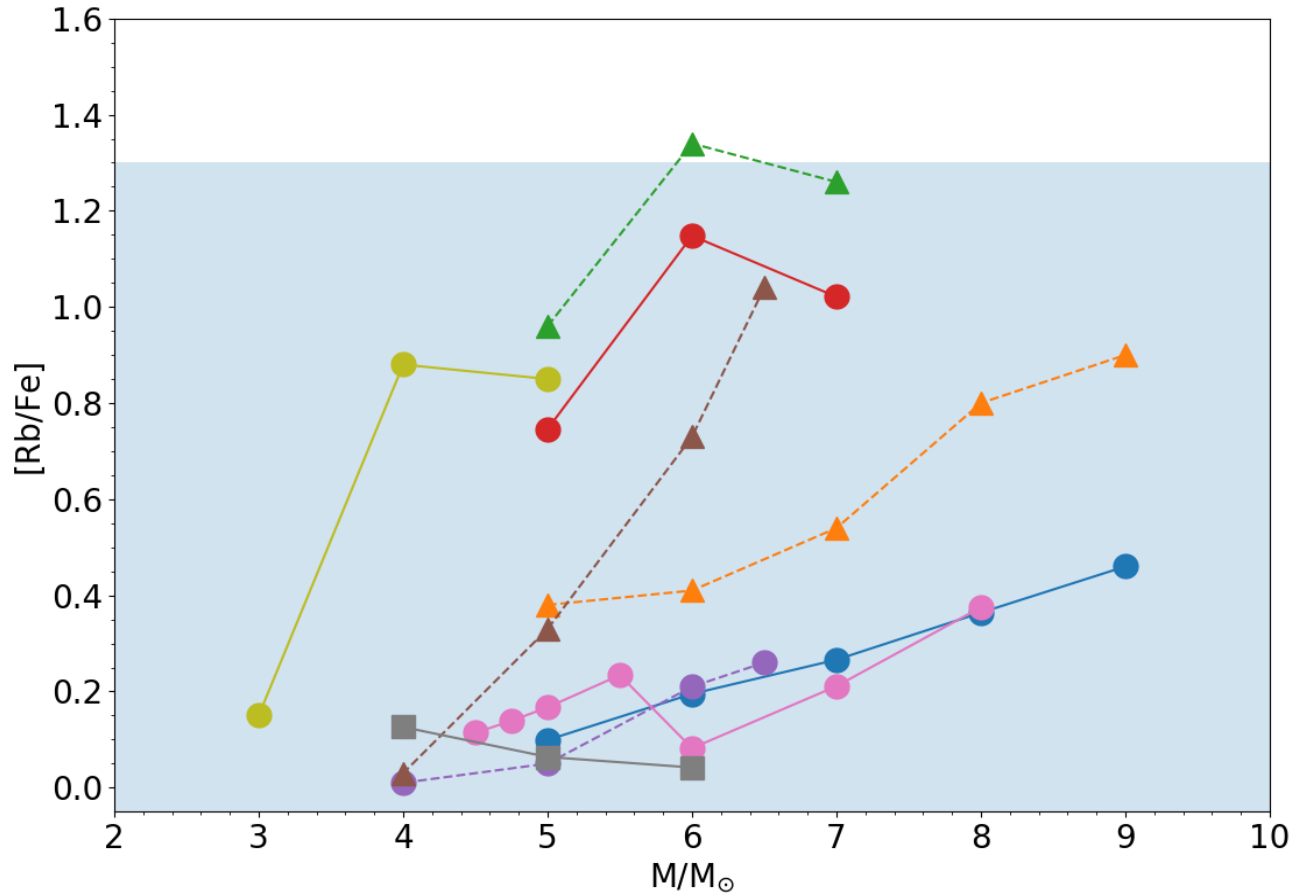
\includegraphics[width=5.0in]{Chapter-3/figs/RbProblem1.png}
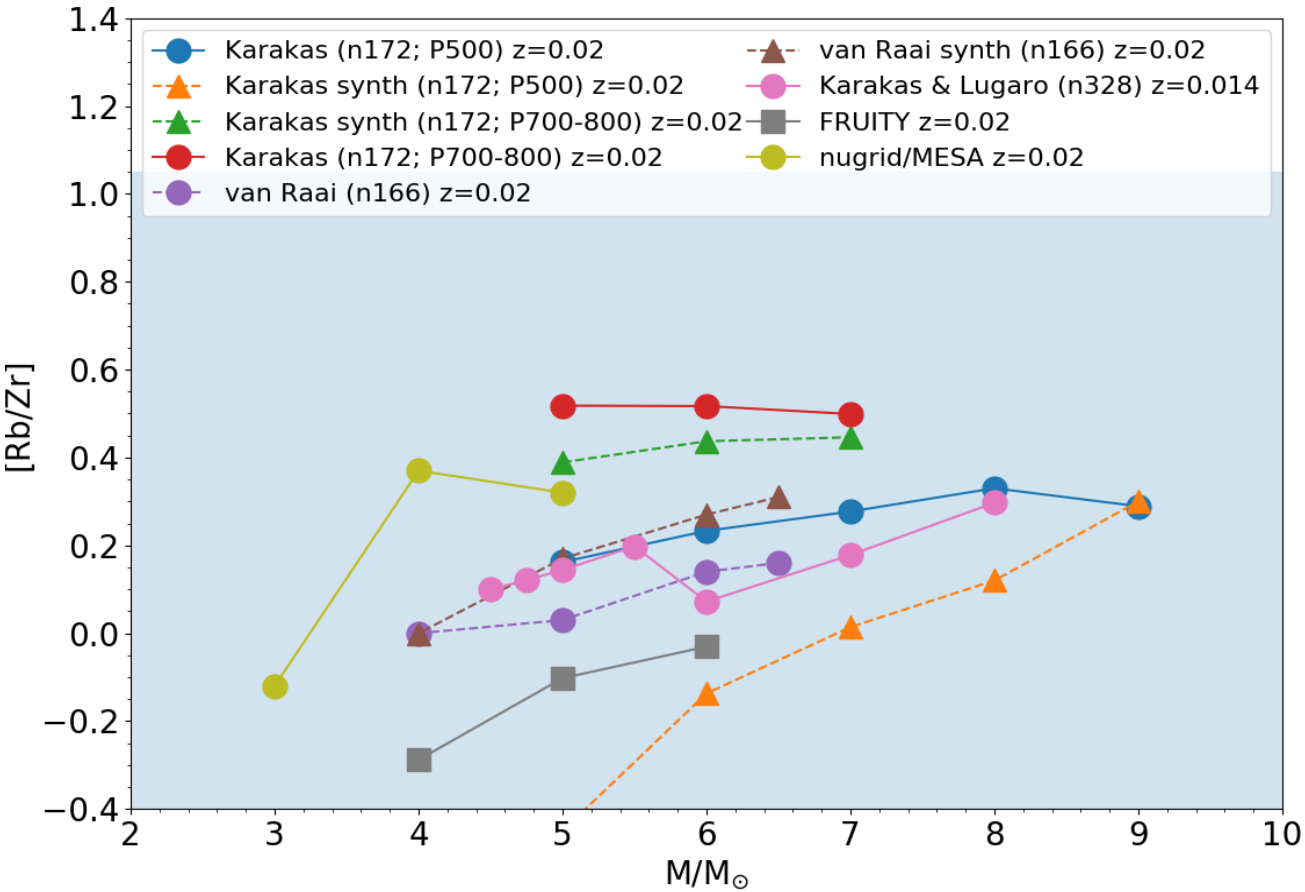
\includegraphics[width=5.0in]{Chapter-3/figs/RbProblem2.png}
\caption{\label{fig:RbProblem}The AGB model predictions of [Rb/Fe] (top) and [Rb/Zr] (bottom) as a function of stellar mass from Refs. \cite{Karakas2012,Raai2012,Karakas2016,Pignatari2016}. The dots and triangles represent abundances from the last computed thermal pulse and from synthetic calculations, respectively. The number of nuclei $n$ in the corresponding network is provided in the legend, as well as the delay superwind parameter $P$ (see text), if applicable, and the metallicity $z$. The range of observed [Rb/Fe] and [Rb/Zr] values from Ref. \cite{Perez2017} are shown by the shaded blue background. Adapted from Ref. \cite{Perez2017}.}
\end{figure}

The analysis that Refs. \cite{Garcia2006,Garcia2007,Garcia2009} performed to obtain the high Rb abundances included the use of a stellar atmospheric model with a classical hydrostatic atmosphere \cite{Gustafsson2008}. Ref. \cite{Zamora2014} developed an updated atmospheric model of AGB stars that incorporated a pseudo-dynamical atmosphere and applied this to a small sample of 5 O-rich AGB stars. They found updated [Rb/Zr] ratios much lower than those obtained with the classical hydrostatic models and in better agreement with the theoretical nucleosynthesis models. Ref. \cite{Perez2017} expanded this study to investigate the full sample of massive Galactic AGB stars analyzed by Refs. \cite{Garcia2006,Garcia2007}. They found a similar decrease in the [Rb/Fe] abundances and [Rb/Zr] ratios, in much better agreement with theoretical models from Refs. \cite{Karakas2012,Raai2012,Karakas2016,Pignatari2016}. 

Figure \ref{fig:RbProblem} shows these theoretical model predictions as a function of AGB mass, compared with the new range of observed [Rb/Fe] abundances (top) and [Rb/Zr] ratios (bottom) from the updated pseudo-dynamical atmospheric models, shaded in blue \cite{Perez2017}. The dots and triangles represent abundances from the last computed thermal pulse and from synthetic calculations, respectively. The models with a modified mass-loss prescription (green and red points), indicated with $P=700-800$ shown in the legend, delay the beginning of the superwind phase until the pulsation period $P$ reaches the indicated number of days. The effect of these models is to intentionally increase the Rb abundance, hence the red and green models show much higher Rb production than the others, which all use the standard $P=500$ days. The full range of the [Rb/Fe] abundances can now be reproduced by the theoretical models, but the largest [Rb/Zr] ratios are still not reproduced. The largest [Rb/Zr] ratio found by Ref. \cite{Perez2017} is 1.05 dex, and the largest of any theoretical model is 0.52 dex, a difference of 0.53 dex. Therefore, despite the better agreement with moderate [Rb/Zr] ratios, the largest observed [Rb/Zr] ratios have still not been reproduced for Galactic O-rich AGB stars. This is true even for the modified AGB models, where Rb abundance is artificially enhanced. In conjunction with this remaining discrepancy, the extreme [Rb/Fe] and [Rb/Zr] observations for O-rich AGB stars in the LMC and SMC \cite{Garcia2009} have yet to be reconciled.

The rubidium problem is investigated in the remainder of this chapter by considering the reaction rate uncertainties of all reactions relevant to the s-process in AGB stars. Some of these reactions are essential to rubidium production in the models presented in this section. In particular, the s-process branching at $^{86}$Rb is investigated with a nuclear reaction network (see Section \ref{sec:nuc_reac_network}) by considering the relative abundance of $^{87}$Rb to the nearby nuclei $^{86}$Sr and $^{90}$Zr. If these ratios are significantly altered when sampling a given reaction rate within its own uncertainty, the reaction is considered significant to rubidium production.

\section{s-Process Reaction Network Methodology} \label{sec:network_method}

\subsection{The Reaction Network} \label{subsec:the_reaction_network}

% Description of the nuclei / reactions in the network (rates from Starlib) and their initial abundances.
% Start off with the simple 47.5% 22Ne, 47.5% 4He, and 5% 85Rb case.
% Then then solar system abundances case, where 1H --> 4He and 12C+13C --> 14N

An s-process reaction network of 769 nuclei and 7,571 reactions from $^{1}$H to $^{212}$Bi is considered, where nucleosynthesis is simulated during a single thermal pulse in the intershell region of an AGB star at constant temperature $T$ and density $\rho$. The system of differential equations described by Eqn. \ref{eqn:AbundEvol_General} is computed numerically, given the reaction rate probability densities tabulated in the \texttt{Starlib} \cite{Sallaska2013} library, truncated for the nuclei in the network. The median, recommended reaction rates are used for the single calculation described in Section \ref{subsec:abund_evol}, while the full probability densities are sampled in Section \ref{sec:rate_sensitivities}. The abundances at each time step are reported in terms of mass fractions $X$. The final time is determined by the amount of helium that has been exhausted, such that a final mass fraction of $X_{\mathrm{last}}(^{4}\mathrm{He})$ stops the evolution. Helium is not expected to be completely exhausted during a thermal pulse, so this condition is chosen to be slightly less than the initial $^{4}$He mass fraction $X_{\mathrm{init}}(^{4}\mathrm{He})$.

The intershell region consists of about $75\%$ $^{4}$He, $22\%$ $^{12}$C, and a small amount of $^{16}$O \cite{Habing2004}, with the remainder roughly approximated in terms of relative solar system abundances \cite{Lodders2009}. A complication to consider is how to address proton-mixing because it is not inherently described by Eqn. \ref{eqn:AbundEvol_General}, yet it is the origin of the neutron sources $^{13}\mathrm{C}(\alpha,n)^{16}\mathrm{O}$ and $^{22}\mathrm{Ne}(\alpha,n)^{25}\mathrm{Mg}$ via the $^{13}$C and $^{14}$N pockets, respectively. Additionally, no protons are expected to exist in the intershell region during thermal pulses, as they get consumed in the formation of the $^{13}$C and $^{14}$N pockets. This issue is rectified by enhancing the initial mass fractions of $^{13}$C and $^{14}$N from their relative solar system abundances to simulate the $^{13}$C and $^{14}$N pockets and having an initial $^{1}$H mass fraction of zero. The abundance of the $^{56}$Fe s-process seed nucleus is also slightly enhanced from its relative solar system abundance, to achieve a more efficient s-process. The initial abundances used in the present reaction network are provided in Table \ref{tab:init_abunds}.

The constant temperature $T$ and density $\rho$ for the reaction network are chosen as 300 MK and $10^{3}$ $\mathrm{g}/\mathrm{cm}^{3}$, respectively, indicative of the conditions in the intershell region during a thermal pulse at which the $^{22}\mathrm{Ne}(\alpha,n)^{25}\mathrm{Mg}$ neutron source is expected to activate \cite{Habing2004}. The $X_{\mathrm{last}}(^{4}\mathrm{He})$ parameter is chosen as 0.7, where $X_{\mathrm{init}}(^{4}\mathrm{He}) = 0.75$.

\subsection{Abundance Evolution} \label{subsec:abund_evol}

% Abundance evolution plots of 87Rb, 88Sr, Kr isotopes, 4He, 14N, 13C, etc.

The abundance evolution for a single s-process nuclear reaction network calculation is shown in Fig. \ref{fig:abund_evol}. It is apparent that $^{13}$C and $^{14}$N suddenly drop just after $10^{3}$ s, corresponding with a burst of neutrons $n$. $^{16}$O and $^{25}$Mg production occur simultaneously, indicating that the neutron sources $^{13}\mathrm{C}(\alpha,n)^{16}\mathrm{O}$ and $^{22}\mathrm{Ne}(\alpha,n)^{25}\mathrm{Mg}$ are active, respectively. This burst of neutrons leads to a production of $^{87}$Rb and a destruction of the initial $^{86}$Sr, indicating that the neutron density is sufficient to active the $^{85}$Kr and $^{86}$Rb s-process branchings.

The flux plot of Fig. \ref{fig:Flux} tells a slightly more nuanced story. In the plot, arrows indicate the reactions that have occurred in the network, producing a net abundance flow from one nucleus to another. The arrow thickness is associated with the magnitude of the integrated flux, with three levels of relative magnitude depicted. The reactions with the largest net flux are the triple-$\alpha$ reaction, the $^{13}$C neutron source sequence $^{12}\mathrm{C}(p,\gamma)^{13}\mathrm{N}(\beta^{+}\nu)^{13}\mathrm{C}(\alpha,n)^{16}\mathrm{O}$ and the neutron poison $^{14}\mathrm{N}(n,p)^{14}\mathrm{C}$. The $^{22}$Ne neutron source sequence $^{14}\mathrm{N}(\alpha,\gamma)^{18}\mathrm{F}(\beta^{+}\nu)^{18}\mathrm{O}(\alpha,\gamma)^{22}\mathrm{Ne}$ is present, but it is associated with the middle tier of relative magnitude. Hence, the $^{13}$C neutron source appears to be the dominant one, even though the s-process branchings clearly favor $^{87}$Rb from the abundance evolution of Fig. \ref{fig:abund_evol}. Interestingly, the $^{13}\mathrm{N}(n,p)^{13}\mathrm{C}$ net flux, overlapping with that of $^{13}\mathrm{N}(\beta^{+}\nu)^{13}\mathrm{C}$, is also quite large, destroying neutrons along with $^{14}\mathrm{N}(n,p)^{14}\mathrm{C}$. The protons produced from these reactions likely contribute to the $^{12}\mathrm{C}(p,\gamma)^{13}\mathrm{N}$ reaction, giving rise to more $^{13}$C, even though no initial protons were provided.

\begin{figure}[t]
\centering
\begin{tikzpicture}[scale=0.8, every node/.style={transform shape}]
\node at (0,0) {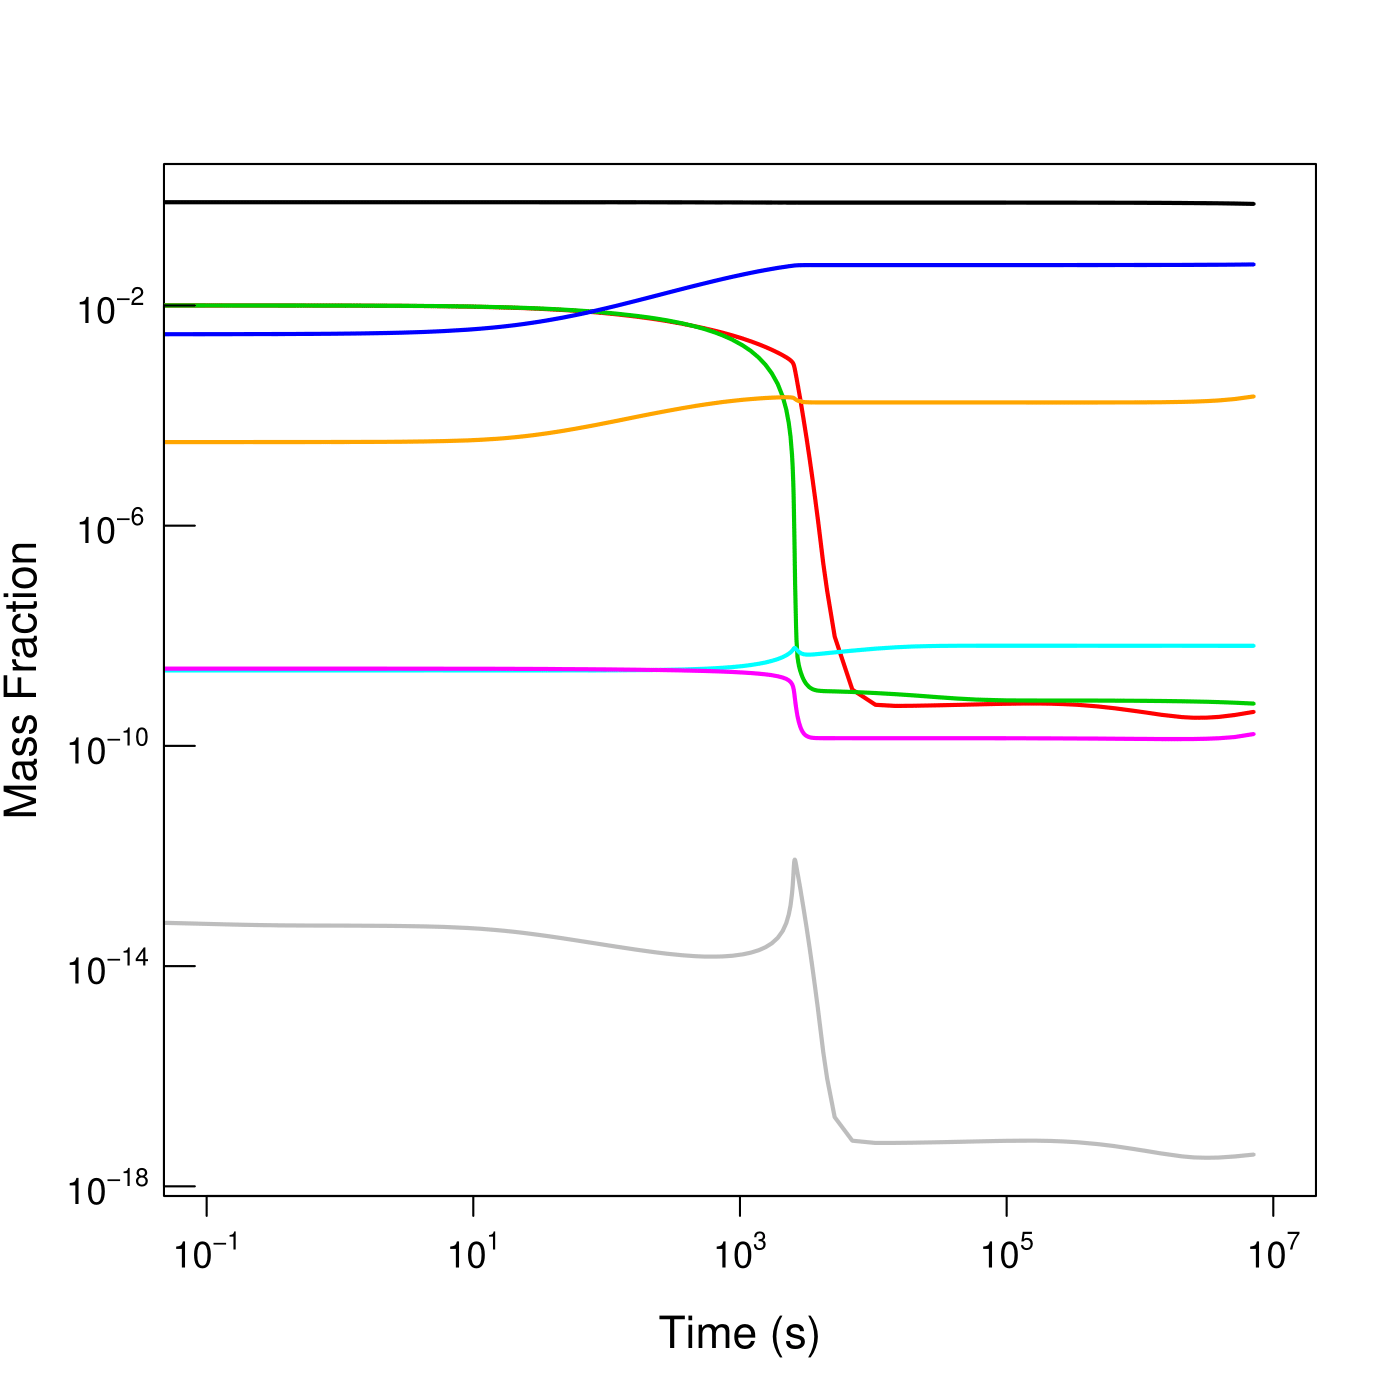
\includegraphics[width=6.5in]{Chapter-3/figs/abund_evol.png}};
\node at (-1.5,5.6) {$^{4}$He};
\node at (1.8,2) {$^{13}$C};
\node at (0.7,2) {$^{14}$N};
\node at (3,4.75) {$^{16}$O};
\node at (5,3.1) {$^{25}$Mg};
\node at (4,1.0) {$^{87}$Rb};
\node at (4,-0.8) {$^{86}$Sr};
\node at (1.75,-3.5) {$n$};
\node[draw] at (-3,-5) {$T = 300$ MK, $\rho = 10^{3}$ $\mathrm{g}/\mathrm{cm}^{3}$};
\end{tikzpicture}
\caption{\label{fig:abund_evol}The abundance evolution of key nuclei related to the s-process branching at $^{86}$Rb for a single network calculation simulating the conditions during a single AGB thermal pulse. The $T$, $\rho$, and $X_{\mathrm{last}}(^{4}\mathrm{He})$ parameters are 300 MK, $10^{3}$ $\mathrm{g}/\mathrm{cm}^{3}$, and 0.7, respectively, with $X_{\mathrm{init}}(^{4}\mathrm{He}) = 0.75$.}
\end{figure}

A test of the initial abundances was performed where the enhanced value of $X_{\mathrm{init}}(^{13}\mathrm{C}) = 0.01$ was swapped with the solar system value of $X_{\mathrm{init}}(^{22}\mathrm{Ne}) = 6.34 \times 10^{-5}$, in order to see if the $^{22}\mathrm{Ne}(\alpha,n)^{25}\mathrm{Mg}$ neutron source could be maximized and the $^{13}\mathrm{C}(\alpha,n)^{16}\mathrm{O}$ neutron source could be minimized. Indeed, the net flux of $^{22}\mathrm{Ne}(\alpha,n)^{25}\mathrm{Mg}$ increases, but not as significantly as one might expect, since the two neutron sources have roughly equivalent flux in this scenario. In addition, the final $X(^{87}\mathrm{Rb})/X(^{86}\mathrm{Sr})$ ratio decreases with these initial abundances, presumably from the drop in neutron density as a result of the weaker $^{13}\mathrm{C}(\alpha,n)^{16}\mathrm{O}$ flux. Increased temperatures were also tested, but the abundance evolution is considerably more complicated, yet the fluxes remained more or less consistent, with only slight enhancements in the $^{14}\mathrm{N}(\alpha,\gamma)^{18}\mathrm{F}(\beta^{+}\nu)^{18}\mathrm{O}(\alpha,\gamma)^{22}\mathrm{Ne}$ sequence. The topic of $X_{\mathrm{init}}$, $T$, and $\rho$ variations merits further investigation, but the simple s-process model described in Figs. \ref{fig:abund_evol} and \ref{fig:Flux} is sufficient for the present purpose of investigating reactions important to rubidium production, as the $^{85}$Kr and $^{86}$Rb s-process branchings are clearly activated.

\begin{figure}[t]
\centering
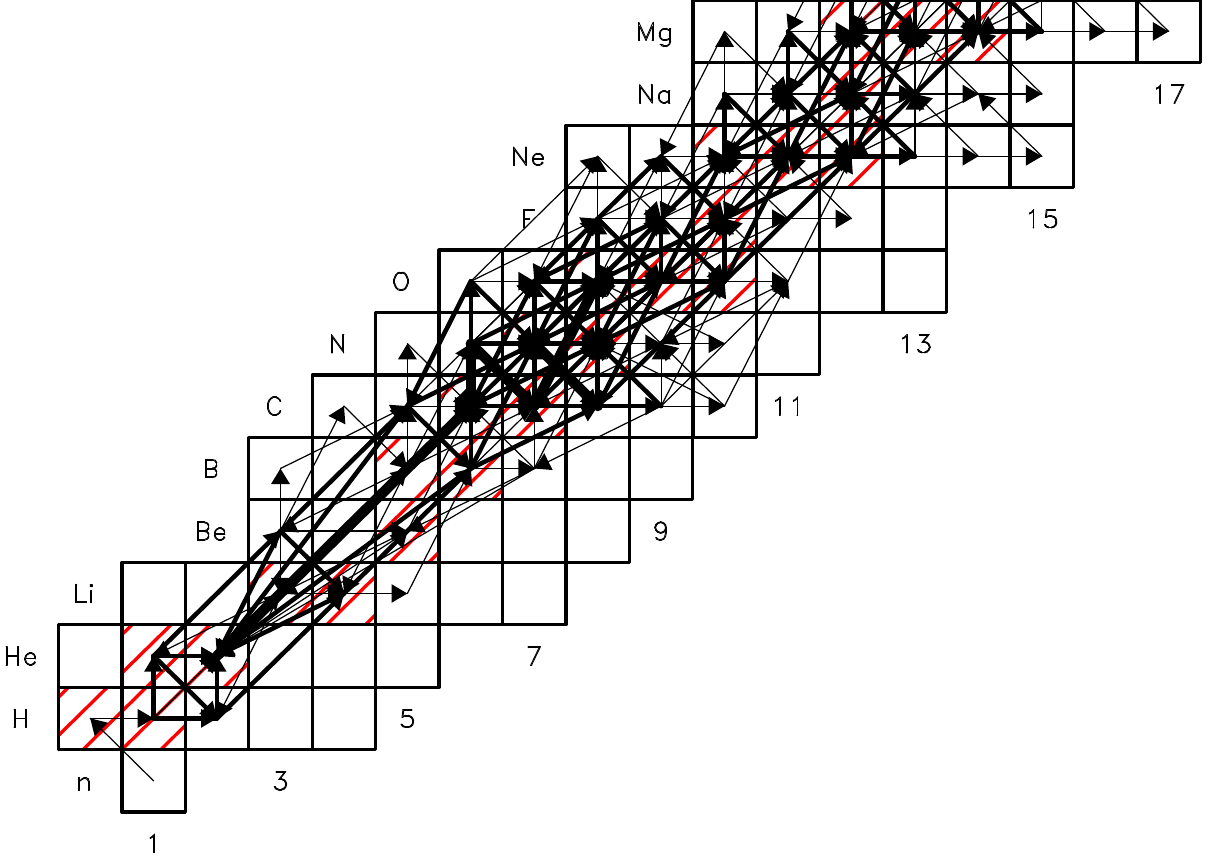
\includegraphics[width=6.5in]{Chapter-3/figs/Flux.png}
\caption{\label{fig:Flux}The network flux plot for a single network calculation simulating the conditions during a single AGB thermal pulse. The $T$, $\rho$, and $X_{\mathrm{last}}(^{4}\mathrm{He})$ parameters are 300 MK, $10^{3}$ $\mathrm{g}/\mathrm{cm}^{3}$, and 0.7, respectively, with $X_{\mathrm{init}}(^{4}\mathrm{He}) = 0.75$. The arrow thickness corresponds to the magnitude of the integrated flux from one nucleus to another, with three levels of relative magnitude shown. The reactions with the largest net flux are the triple-$\alpha$ reaction, the $^{13}$C neutron source sequence $^{12}\mathrm{C}(p,\gamma)^{13}\mathrm{N}(\beta^{+}\nu)^{13}\mathrm{C}(\alpha,n)^{16}\mathrm{O}$, and the neutron poison $^{14}\mathrm{N}(n,p)^{14}\mathrm{C}$.}
\end{figure}

\subsection{Monte Carlo Procedure}

% Explanation of the Monte Carlo reaction network calculations

% Longland2012 (reaction rate sampling), Iliadis2015b (Pearson's and Spearman's correlations), and Iliadis2020  (mutual information)

The reaction rate probability densities of \texttt{Starlib} \cite{Sallaska2013}, calculated with the \texttt{RatesMC,RatesMC} code \cite{Longland2010a}, are sampled in the remaining analysis of this chapter. The reaction rates in the network are varied simultaneously based on these samples, and a single network calculation is performed with the new rates leading to a new array of final abundances. This procedure is performed for several thousand samples, and the final abundances therefore form probability densities of their own. These reaction rates are calculated given nuclear physics inputs, which can contain large uncertainties. To properly sample these uncertainties, a Monte Carlo sampling procedure is the most efficient. This procedure is described by Ref. \cite{Longland2012}, and a summary is presented here. 

The rate probability densities in \texttt{Starlib} are described by the lognormal shape parameters $\mu$ and $\sigma$ (not to be confused with the gaussian mean and standard deviation),
\begin{align} \label{eqn:lognorm_param}
\mu &= \ln x_{\mathrm{med}}, \nonumber \\
\sigma &= \ln \sqrt{\frac{x_{\mathrm{high}}}{x_{\mathrm{low}}}}, 
\end{align} 
where $x_{\mathrm{med}}$, $x_{\mathrm{high}}$, and $x_{\mathrm{low}}$ are the median (recommended), 84th percentile, and 16th percentile rates, respectively. Reaction rate samples $x(T)_{i}$ are drawn from a given reaction $j$ at the temperature $T$ and are represented by
\begin{align} \label{eqn:MC_Sampling}
x(T)_{ij} &= e^{\mu(T)_{j}} \, e^{p(T)_{ij} \sigma(T)_{j}} \nonumber \\
&= x(T)_{\mathrm{med},j}\left[ f.u.(T) \right]^{p(T)_{ij}}_{j},
\end{align}
where $p(T)$ is a gaussian-distributed random variable with a mean of zero and a standard deviation of unity, known as the \emph{rate variation factor}, and the factor $f.u.(T) \equiv e^{\sigma(T)}$ is known as the \emph{factor uncertainty}. The parametrization of $p(T)$ can be treated as independent of temperature to an excellent approximation \cite{Longland2012}, known as a flat parametrization, $p(T) = p$. In this scenario, $p$ is sampled from a normal distribution, but $f.u.(T)$ remains a temperature-dependent quantity due to the lognormal $\sigma(T)$ parameter. If $f.u.$ were independent of temperature, then the entire reaction rate would be varied regardless of the uncertainty temperature dependence. This is a bad approximation for experimentally-constrained reaction rates, where the uncertainty is very temperature-dependent. Since the present reaction network model uses a constant $T = 300$ MK though, only the rate uncertainty at this temperature needs to be sampled. Additionally, forward and reverse reaction rates are not sampled independently, as the same value of $p$ is applied to both rates.

\subsection{Measuring Correlations with Mutual Information}

% Explanation of the Spearman, Pearson, and mutual information statistics
One of the primary goals in performing Monte Carlo reaction network calculations is to determine which reaction rates would benefit from experimental constraint for the given nucleosynthesis model. If the abundances of key nuclei are significantly altered when varying a reaction rate within its probability density, that rate is likely significant to the present nucleosynthesis.
%, or it has a large uncertainty in the given temperature range, or both. This point is stressed here because some important reaction rates may not affect the abundances of key nuclei when they are varied within their uncertainties because the uncertainties are sufficiently small. If a constant temperature $T$ is used in the Monte Carlo network calculation, it can also highlight which reaction rates are not very well constrained at $T$.
The reaction rate sensitivity of a given reaction $j$ on the abundance of a given nucleus can be determined by analyzing the scatter plot between the rate variation factor $p_{j}$ and the final mass fraction $X$ over all network samples \cite{Iliadis2015b}. This can also be performed for an abundance ratio of nuclei $1$ and $2$ with the mass fraction ratio $X_{1}/X_{2}$. The random variables $p_{j}$ and $X$ are recorded after each network sample, and correlations are determined during post-processing using one of a variety of statistical metrics. For a given key mass fraction $X$ or mass fraction ratio $X_{1}/X_{2}$, the correlations are then ranked according to this metric to determine the most important reaction rates governing the nucleosynthesis.

Pearson's correlation coefficient $r$ has been used by Ref. \cite{Coc2014} to determine the linearity of these two random variables for reactions sensitive to $^{6}$Li production in big bang nucleosynthesis. However, this metric is not effective when the correlation is nonlinear. Spearman's correlation coefficient $r_{s}$ was used by Ref. \cite{Iliadis2015b} for a similar nucleosynthesis network. It is more effective at quantifying nonlinear correlations because it measures the relationship between two variables described by a monotonic function. However, often these correlations are found exhibiting nonlinear behavior and are non-monotonic. A metric that is suitable for a general range of correlations is \emph{mutual information}, recently used by Ref. \cite{Iliadis2020}, which measures the amount of information about one random variable contained in another random variable \cite{Cover2006}. For the discrete random variables $x$ and $y$ containing the values $\{x_{1}, \, x_{2}, \, \ldots\}$ and $\{y_{1}, \, y_{2}, \, \ldots\}$ their mutual information MI is defined as
\begin{equation} \label{eqn:mutual_info}
\mathrm{MI} = \sum_{x} \sum_{y} P(x,y) \log \left[ \frac{P(x,y)}{P(x)P(y)} \right],
\end{equation}
where $P(x)$ and $P(y)$ are the marginal probability distributions of $x$ and $y$, respectively, and $P(x,y)$ is their joint probability distribution. Mutual information between $x$ and $y$ is zero if, and only if, they are independent of each other. This metric has no finite upper limit, meaning the effective use of MI is to compare between relative magnitudes. That is all that is required for the purpose of ranking reaction rate correlations, and we therefore adopt MI as the correlation metric in the present analysis.

\section{Reaction Rate Sensitivities} \label{sec:rate_sensitivities}

\subsection{Correlations} \label{subsec:Corr}

The Monte Carlo reaction network calculation was performed for $5 \times 10^{4}$ samples. Correlations between every reaction in the network and the mass fraction ratios $X(^{87}\mathrm{Rb})/X(^{86}\mathrm{Sr})$ and $X(^{87}\mathrm{Rb})/X(^{90}\mathrm{Zr})$ were computed using the mutual information (MI) metric. The correlations were ranked according to their relative MI values, and the top 8 most correlated reactions rates with each ratio are listed in Table \ref{tab:mutual_info}. Spearman's correlation coefficient $r_{s}$ is provided to indicate the signature (positive or negative) of the correlation, assuming it is at least linear or monotonic. In many cases, the MI and $|r_{s}|$ values are not consistent among the ranks, which is indicative of nonlinear, non-monotonic correlations. The top 3 most correlated reaction rates for both ratios, ranked by MI, are $^{86}\mathrm{Rb}(n,\gamma)^{87}\mathrm{Rb}$, $^{13}\mathrm{N}(n,p)^{13}\mathrm{C}$, and $^{14}\mathrm{N}(n,p)^{14}\mathrm{C}$. The discussion for the latter two reactions will be left for the end of this section, as they require more attention.

Beyond roughly the 8th largest MI values, the correlations slowly approach a minimum, as the reaction rates become increasingly uncorrelated with the mass fraction ratios. For both ratios, the least correlated reaction rate is that of $^{49}\mathrm{V}(\alpha,p)^{52}\mathrm{Cr}$, which has $\mathrm{MI} = 0.0468$ and 0.0311 for $X(^{87}\mathrm{Rb})/X(^{86}\mathrm{Sr})$ and $X(^{87}\mathrm{Rb})/X(^{90}\mathrm{Zr})$, respectively. Hence, the decrease between the top 8 MI values is much sharper than any subsequent decrease, and those reaction rates in Table \ref{tab:mutual_info} are the only ones that have a significant impact when sampling their uncertainties.

\subsubsection{The $^{86}\mathrm{Rb}$ and $^{85}$Kr Branchings}

The $^{86}\mathrm{Rb}(n,\gamma)^{87}\mathrm{Rb}$ rate produces $^{87}$Rb directly from the $^{86}$Rb s-process branching, which also prevents $^{86}$Sr from accumulating, explaining its rank as the strongest correlation with the $X(^{87}\mathrm{Rb})/X(^{86}\mathrm{Sr})$ ratio. Even for the $X(^{87}\mathrm{Rb})/X(^{90}\mathrm{Zr})$ ratio, it has the third strongest correlation. This is likely due to the low neutron-capture cross section of $^{87}$Rb, such that it accumulates when the $^{86}$Rb s-process branching is activated, leading also to a reduced path to Zr.

A large portion of the reaction rates in Table \ref{tab:mutual_info} are associated with the $^{86}$Rb and $^{85}$Kr s-process branchings. The correlation plots for these reaction rates with respect to the $X(^{87}\mathrm{Rb})/X(^{86}\mathrm{Sr})$ ratio are shown in Fig. \ref{fig:Correlations_87Rb86Sr_ng}. The reaction is labeled above each panel, where values of $g$ and (later) $a$ represent $\gamma$ and $\alpha$, respectively. The gaussian-distributed rate variation factor $p$ is given on the $x$-axis, while the indicated mass fraction ratio is given on the $y$-axis. The faint dotted lines show the origin, centered on $p=0$ and the mass fraction ratio of unity. Each red dot is a sample corresponding to a single reaction network calculation. The solid line represents a fit with Spearman's correlation coefficient $r_{s}$, which already fails to capture some of the interesting features, as is the case for the $^{86}\mathrm{Rb}(n,\gamma)^{87}\mathrm{Rb}$ rate in the upper left panel. It is clear that the vertical scatter is quite large, indicative of the fact that all rates are sampled simultaneously to obtain a given mass fraction ratio sample. Despite the scatter, clear correlations are shown. The neutron-capture reactions are associated with a positive correlation, and the $\beta^{-}$ decays, labeled ($\gamma,\gamma$), are associated with a negative correlation. This is the expected behavior, as these reactions are directly responsible for $^{87}$Rb and $^{86}$Sr abundance.

\subsubsection{Reactions Sensitive to $^{87}$Rb/$^{90}$Zr}

Returning to Table \ref{tab:mutual_info}, the $^{90}\mathrm{Y}(n,\gamma)^{91}\mathrm{Y}$ and $^{90}\mathrm{Y}(\beta^{-}\nu)^{90}\mathrm{Zr}$ reaction rates are important only for the $X(^{87}\mathrm{Rb})/X(^{90}\mathrm{Zr})$ ratio. These rates directly affect $^{90}$Zr abundance in opposing ways. The former reaction acts to bypass $^{90}$Zr along the s-process path, while the latter produces it directly. The $r_{s}$ signatures of these rates are indicative of this effect. The $^{87}\mathrm{Kr}(n,\gamma)^{88}\mathrm{Kr}$ reaction rate is also important for the $X(^{87}\mathrm{Rb})/X(^{90}\mathrm{Zr})$ ratio, as it acts to bypass $^{87}$Rb, eventually producing $^{90}$Zr. The neutron-capture reaction rates for $^{86}\mathrm{Rb}(n,\gamma)^{87}\mathrm{Rb}$, $^{85}\mathrm{Kr}(n,\gamma)^{86}\mathrm{Kr}$, $^{90}\mathrm{Y}(n,\gamma)^{91}\mathrm{Y}$, and $^{87}\mathrm{Kr}(n,\gamma)^{88}\mathrm{Kr}$ are shown correlated with $X(^{87}\mathrm{Rb})/X(^{90}\mathrm{Zr})$ in Fig. \ref{fig:Correlations_87Rb90Zr_ng}. Here, the vertical scatter is reduced, likely because $^{90}$Zr is much easier to accumulate than $^{86}$Sr, closing the gap between $^{87}$Rb abundance. It is also a closed-shell ($N=50$) nucleus, similar to $^{87}$Rb, with a low neutron-capture cross section.

\begin{table}[t]
\centering
\caption{\label{tab:mutual_info}Correlations between the most important reaction rates and the $X(^{87}\mathrm{Rb})/X(^{86}\mathrm{Sr})$ and $X(^{87}\mathrm{Rb})/X(^{90}\mathrm{Zr})$ mass fraction ratios, ranked according to mutual information (MI). Spearman's correlation coefficient $r_{s}$ is also provided, to indicate the polarity of the correlation.}
\begin{tabular}{cccc|cccc}
\hline\midrule
\multicolumn{4}{c}{$X(^{87}\mathrm{Rb})/X(^{86}\mathrm{Sr})$}&
\multicolumn{4}{c}{$X(^{87}\mathrm{Rb})/X(^{90}\mathrm{Zr})$}\\
\cmidrule[0.05pt](l{0.5em}r{.9em}){1-4} \cmidrule[0.1pt](l{0.6em}r{.8em}){5-8}
Rank&Reaction&MI&$r_{s}$&Rank&Reaction&MI&$r_{s}$\\ \midrule
1&$^{86}\mathrm{Rb}(n,\gamma)^{87}\mathrm{Rb}$&0.1967&0.4347
&1&$^{13}\mathrm{N}(n,p)^{13}\mathrm{C}$&0.1921&-0.4822\\
2&$^{13}\mathrm{N}(n,p)^{13}\mathrm{C}$&0.1718&-0.4450
&2&$^{14}\mathrm{N}(n,p)^{14}\mathrm{C}$&0.1331&0.1574\\
3&$^{14}\mathrm{N}(n,p)^{14}\mathrm{C}$&0.1341&0.1518
&3&$^{86}\mathrm{Rb}(n,\gamma)^{87}\mathrm{Rb}$&0.1046&0.1405\\
4&$^{85}\mathrm{Kr}(\beta^{-}\nu)^{85}\mathrm{Rb}$&0.1102&-0.2433
&4&$^{90}\mathrm{Y}(n,\gamma)^{91}\mathrm{Y}$&0.1039&0.3222\\
5&$^{86}\mathrm{Rb}(\beta^{-}\nu)^{86}\mathrm{Sr}$&0.1045&-0.2421
&5&$^{87}\mathrm{Kr}(n,\gamma)^{88}\mathrm{Kr}$&0.0741&-0.2138\\
6&$^{85}\mathrm{Kr}(n,\gamma)^{86}\mathrm{Kr}$&0.0951&0.2176
&6&$^{85}\mathrm{Kr}(n,\gamma)^{86}\mathrm{Kr}$&0.0637&0.1973\\
7&$^{18}\mathrm{O}(\alpha,n)^{21}\mathrm{Ne}$&0.0780&0.1272
&7&$^{90}\mathrm{Y}(\beta^{-}\nu)^{90}\mathrm{Zr}$&0.0561&-0.1191\\
8&$^{25}\mathrm{Na}(p,\gamma)^{26}\mathrm{Mg}$&0.0660&0.0097
&8&$^{18}\mathrm{O}(\alpha,n)^{21}\mathrm{Ne}$&0.0521&0.1103\\
\hline\hline
\end{tabular}
\end{table}

%\newpage

\begin{figure}[!p]
\centering
\begin{subfigure}[b]{0.495\textwidth}
\centering
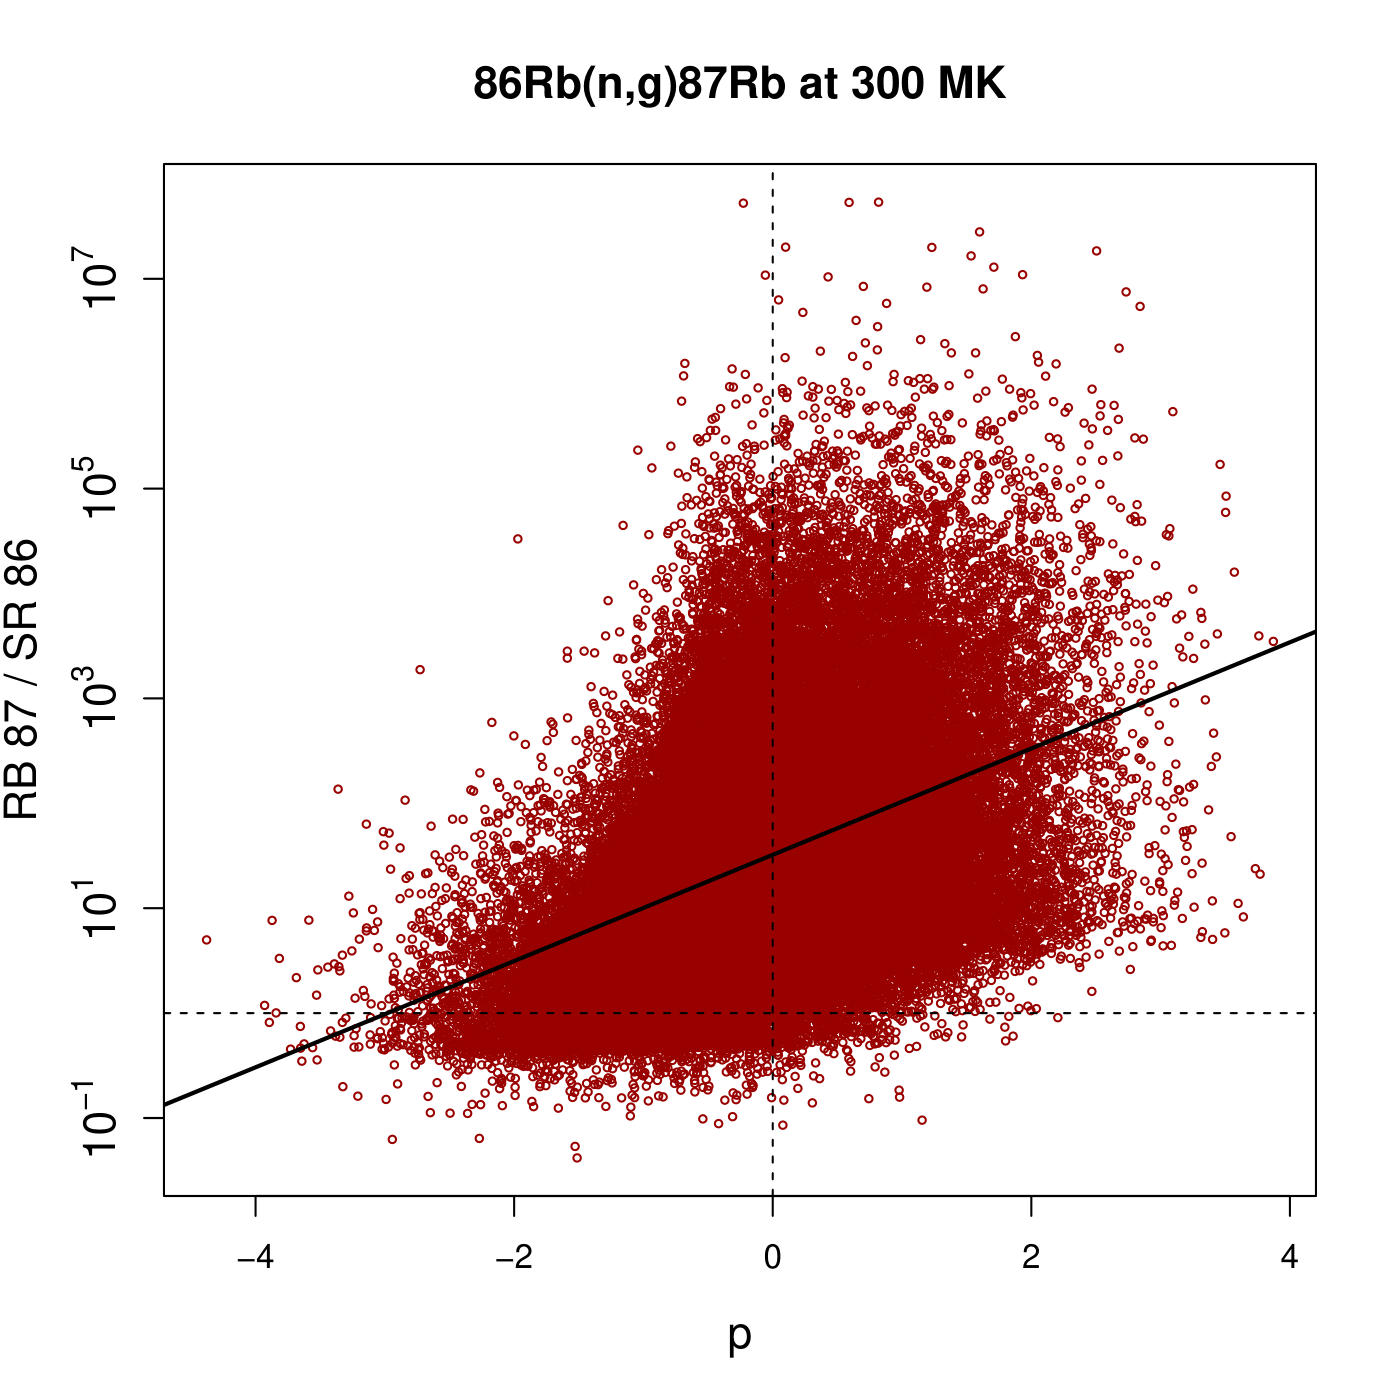
\includegraphics[width=\textwidth]{Chapter-3/figs/CorrRB87SR86_86Rb_n_g_87Rb_300MK.png}  
\end{subfigure}
\hfill
\begin{subfigure}[b]{0.495\textwidth}  
\centering 
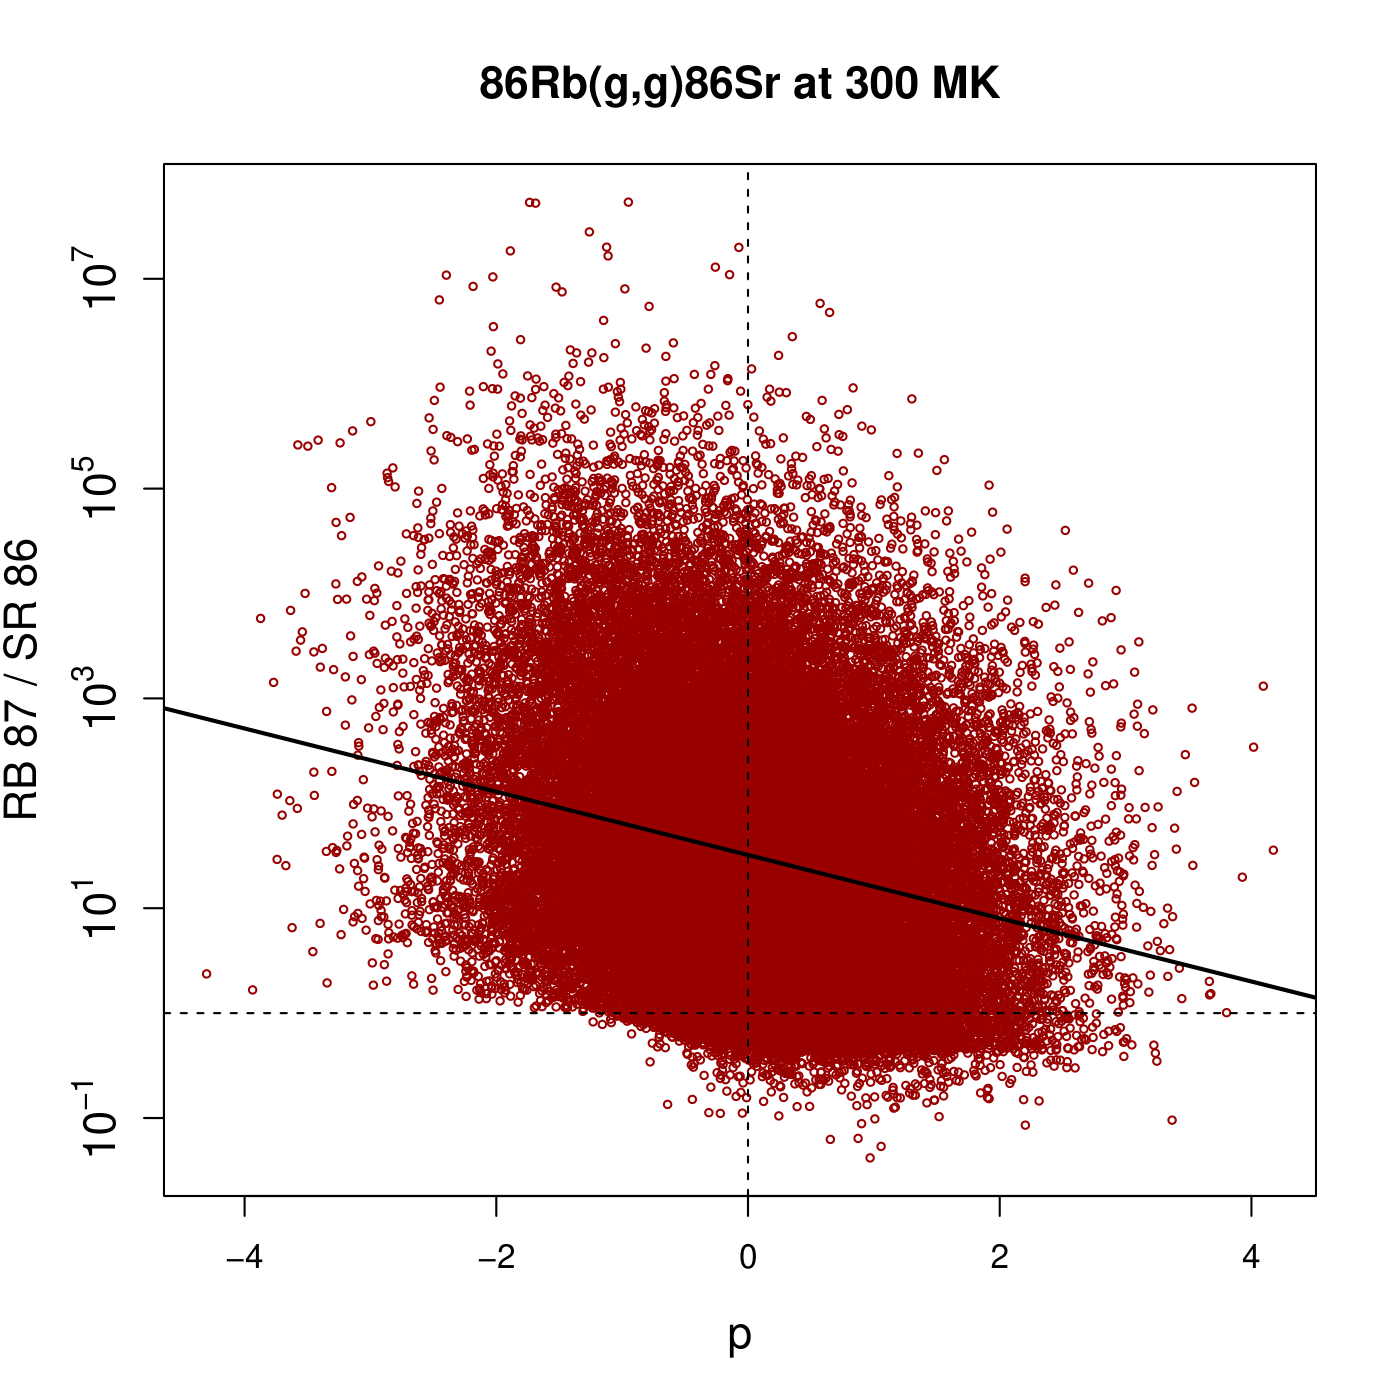
\includegraphics[width=\textwidth]{Chapter-3/figs/CorrRB87SR86_86Rb_g_g_86Sr_300MK.png}
\end{subfigure}
%\vskip\baselineskip
\begin{subfigure}[b]{0.495\textwidth}   
\centering 
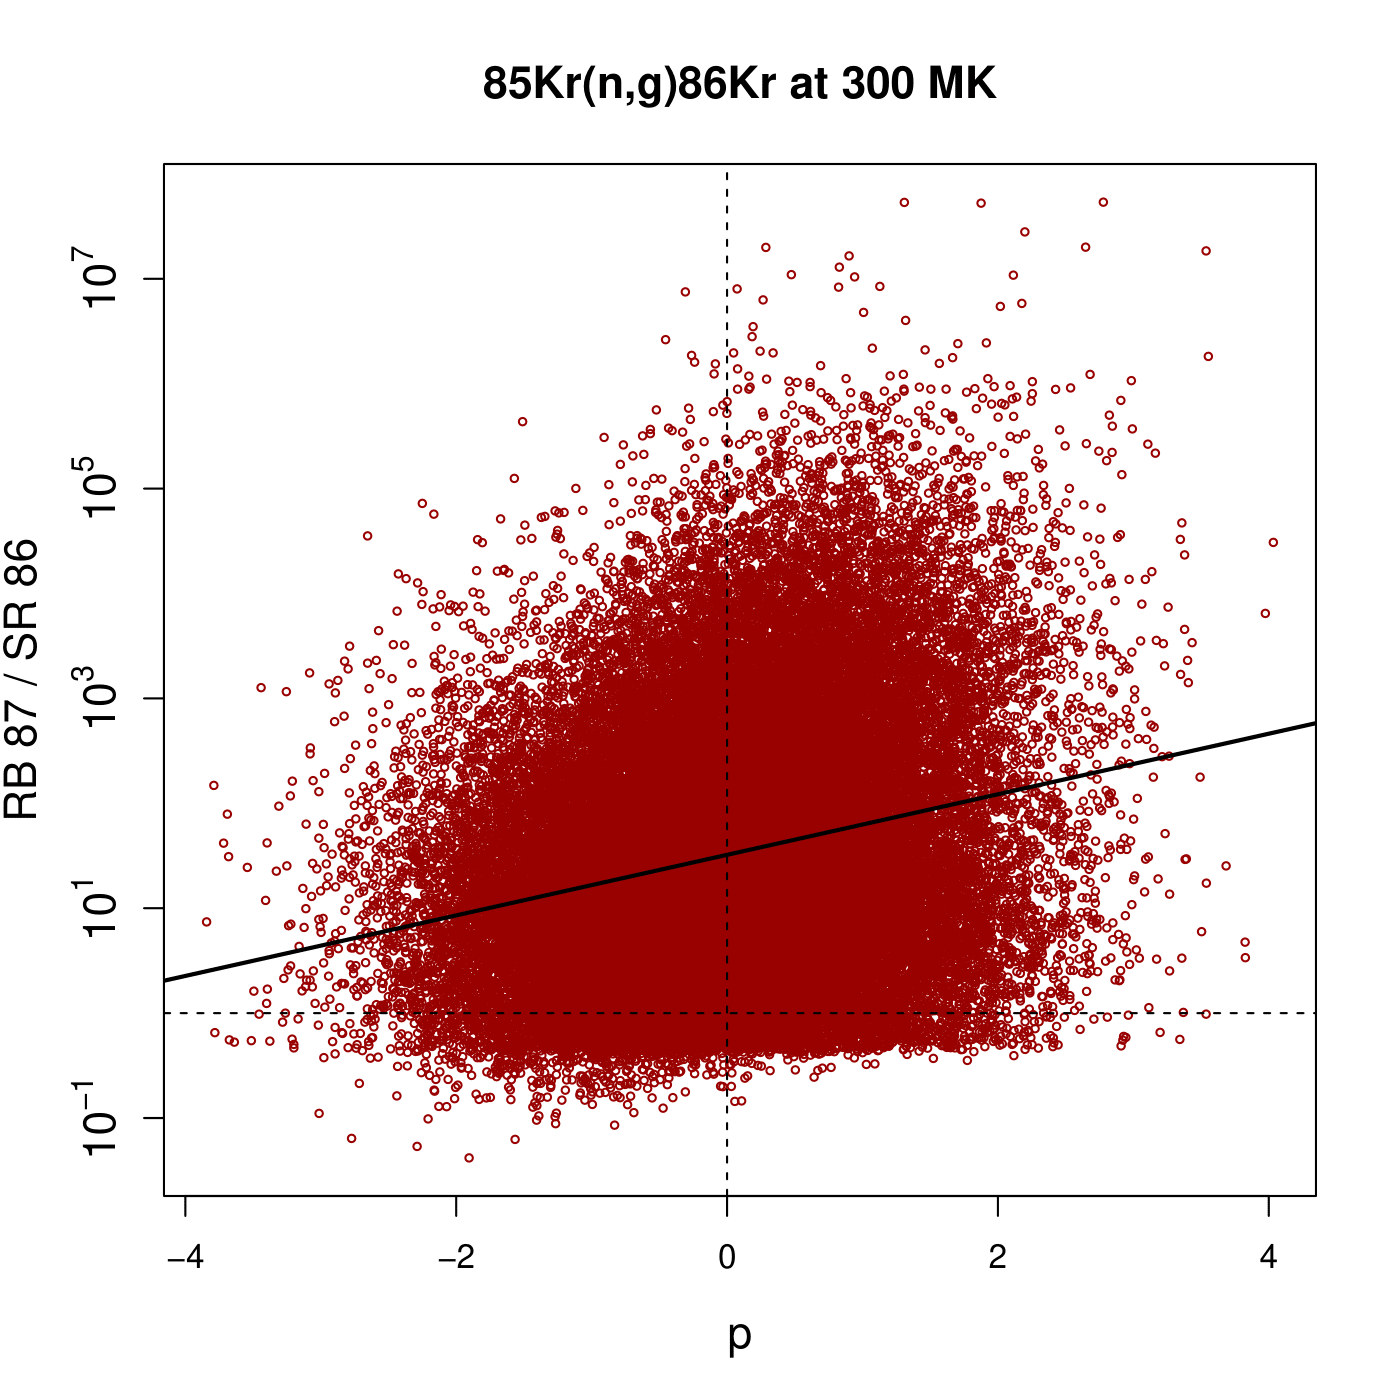
\includegraphics[width=\textwidth]{Chapter-3/figs/CorrRB87SR86_85Kr_n_g_86Kr_300MK.png}
\end{subfigure}
\hfill
\begin{subfigure}[b]{0.495\textwidth}   
\centering 
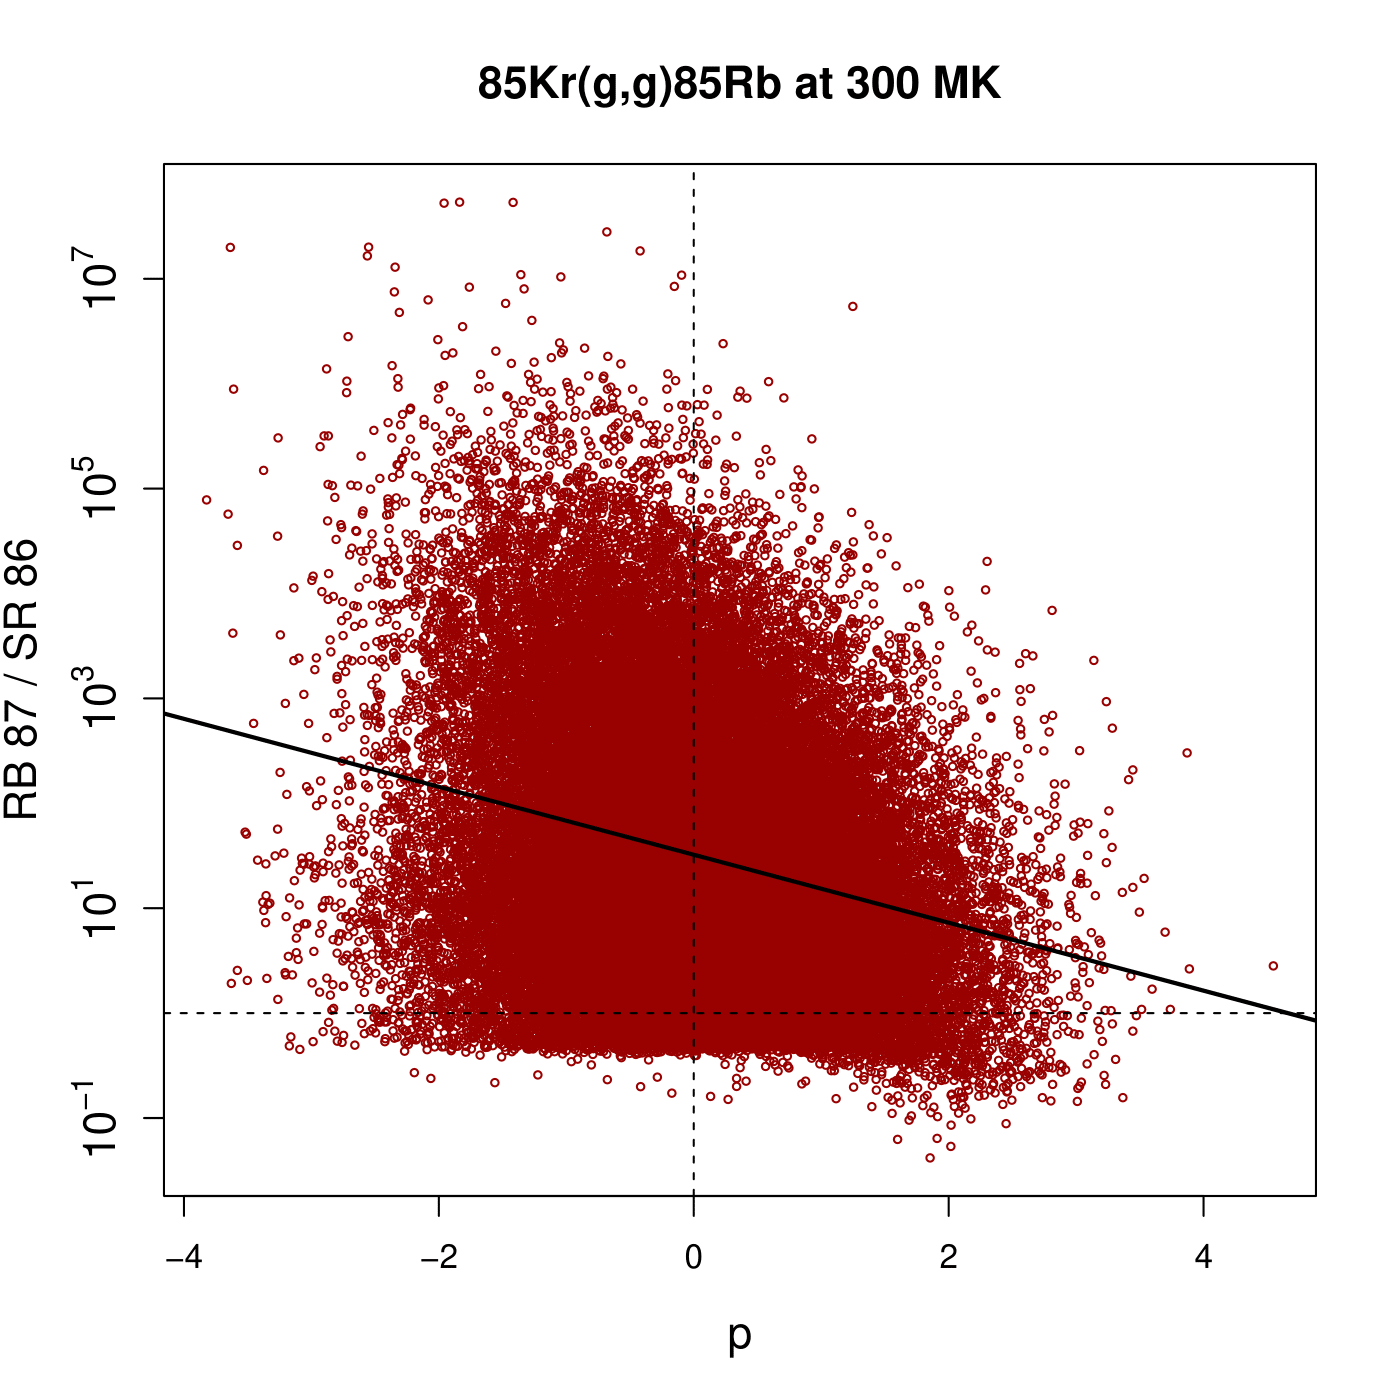
\includegraphics[width=\textwidth]{Chapter-3/figs/CorrRB87SR86_85Kr_g_g_85Rb_300MK.png}
\end{subfigure}
\caption{\label{fig:Correlations_87Rb86Sr_ng}Correlations between the final mass fraction ratio $X(^{87}\mathrm{Rb})/X(^{86}\mathrm{Sr})$ and the important reaction rates of the $^{86}$Rb and $^{85}$Kr s-process branchings, ranked in the top 6 among all reactions by MI. The $x$-axis is given in terms of the gaussian rate variation factor $p$ (see text). The $T$, $\rho$, and $X_{\mathrm{last}}(^{4}\mathrm{He})$ parameters are 300 MK, $10^{3}$ $\mathrm{g}/\mathrm{cm}^{3}$, and 0.7, respectively, with $X_{\mathrm{init}}(^{4}\mathrm{He}) = 0.75$. The Monte Carlo reaction network calculation was performed for $5 \times 10^{4}$ samples. In the title of each plot, the symbols $g$ and (below) $a$ refer to $\gamma$ and $\alpha$, respectively.}
\end{figure}

\begin{figure}[!p]
\centering
\begin{subfigure}[b]{0.495\textwidth}
\centering
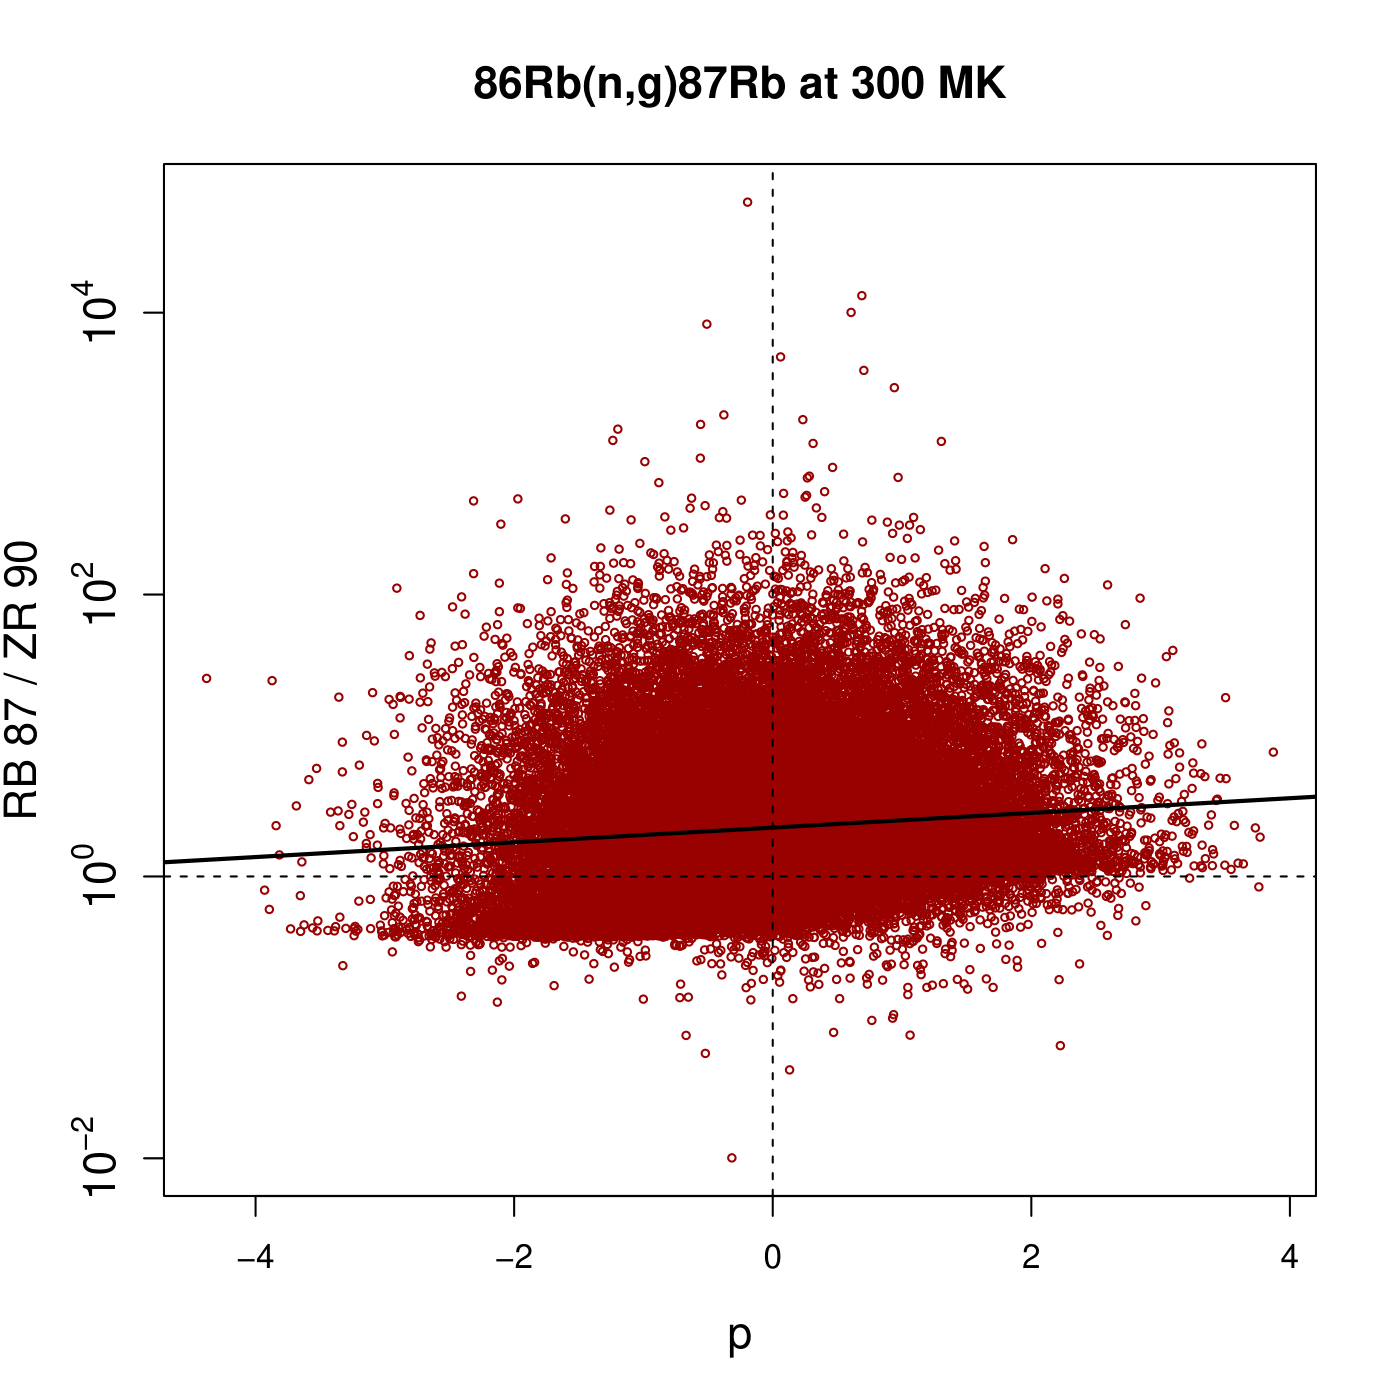
\includegraphics[width=\textwidth]{Chapter-3/figs/CorrRB87ZR90_86Rb_n_g_87Rb_300MK.png}  
\end{subfigure}
\hfill
\begin{subfigure}[b]{0.495\textwidth}  
\centering 
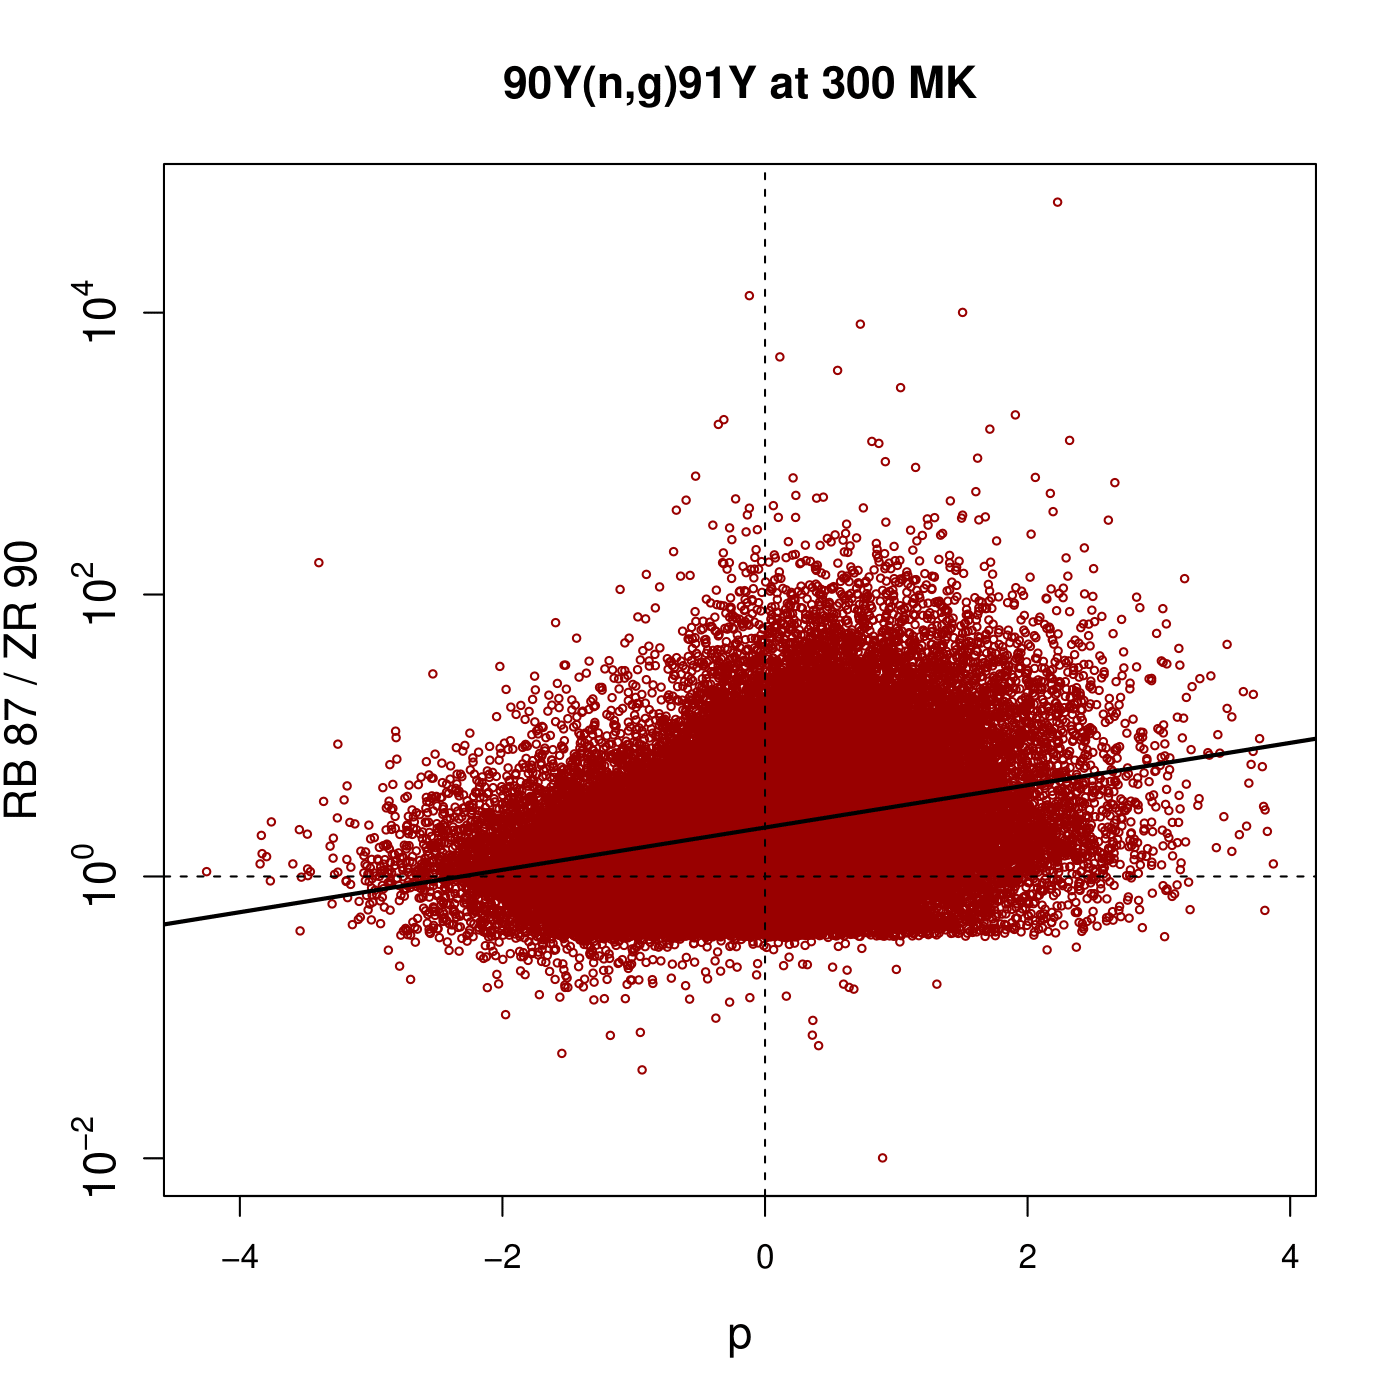
\includegraphics[width=\textwidth]{Chapter-3/figs/CorrRB87ZR90_90Y_n_g_91Y_300MK.png}
\end{subfigure}
%\vskip\baselineskip
\begin{subfigure}[b]{0.495\textwidth}   
\centering 
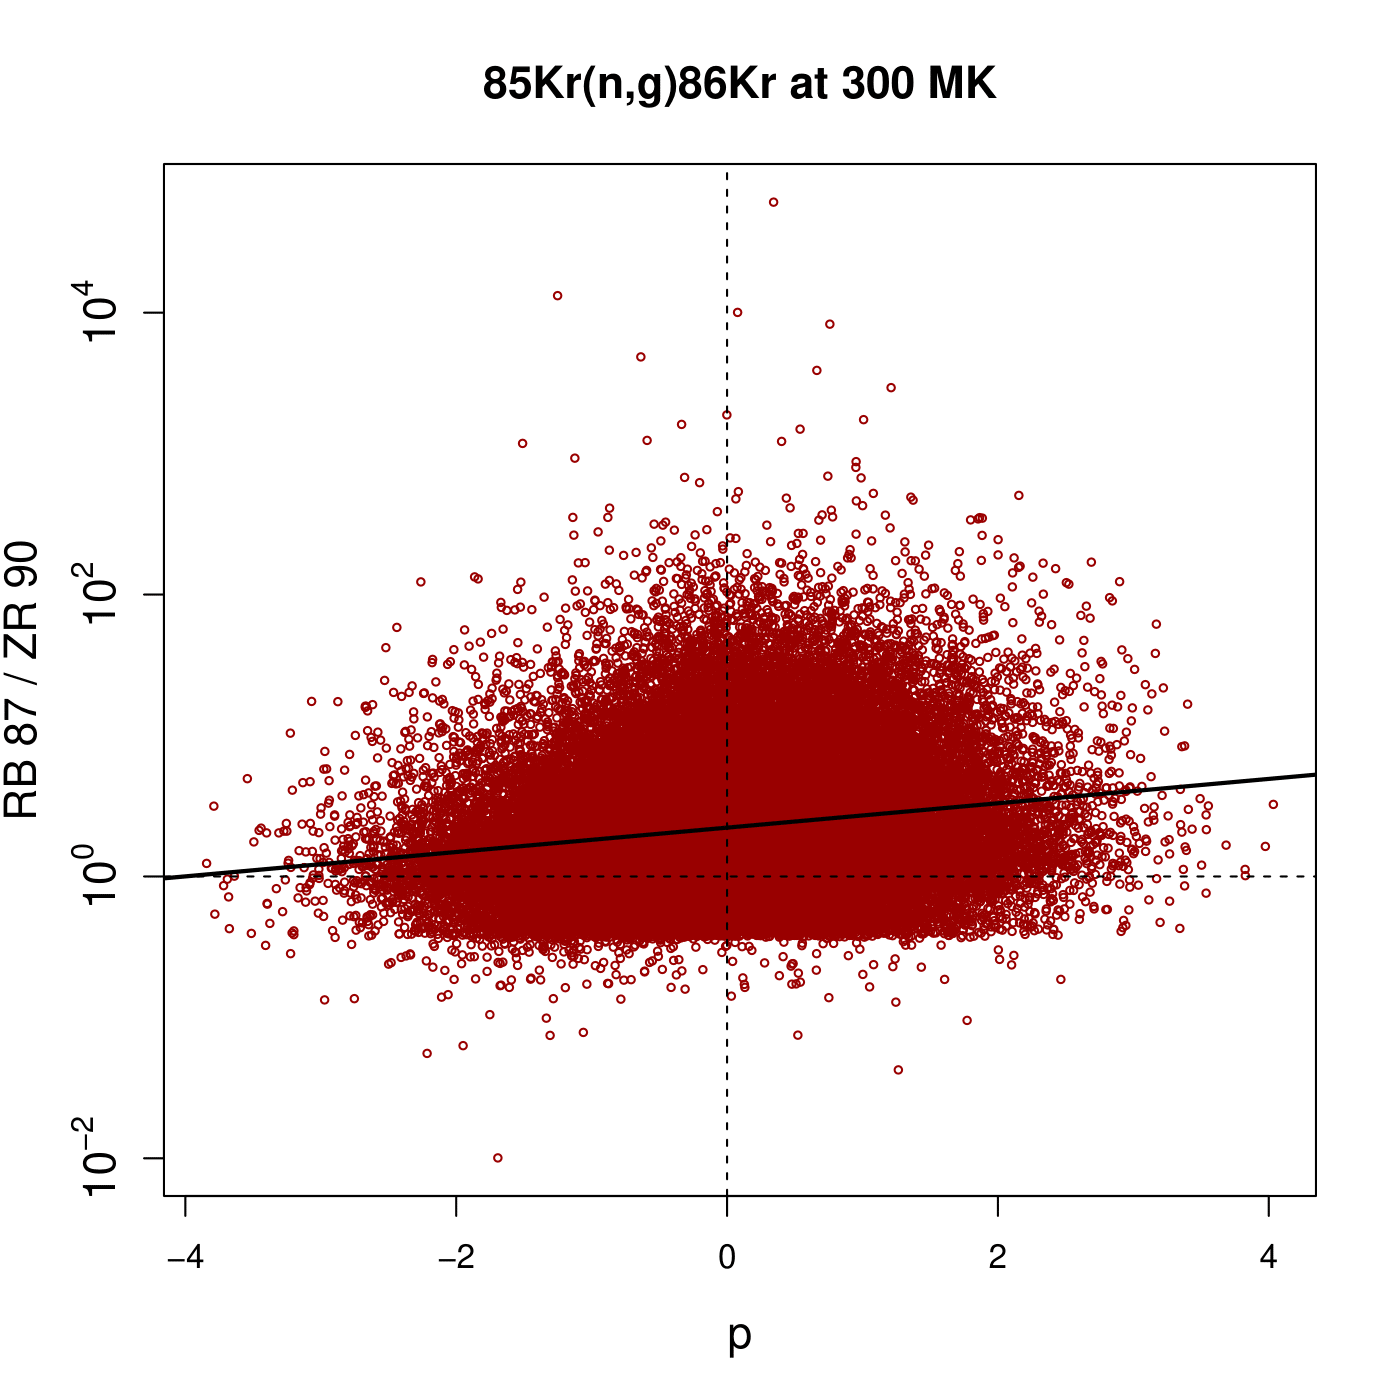
\includegraphics[width=\textwidth]{Chapter-3/figs/CorrRB87ZR90_85Kr_n_g_86Kr_300MK.png}
\end{subfigure}
\hfill
\begin{subfigure}[b]{0.495\textwidth}   
\centering 
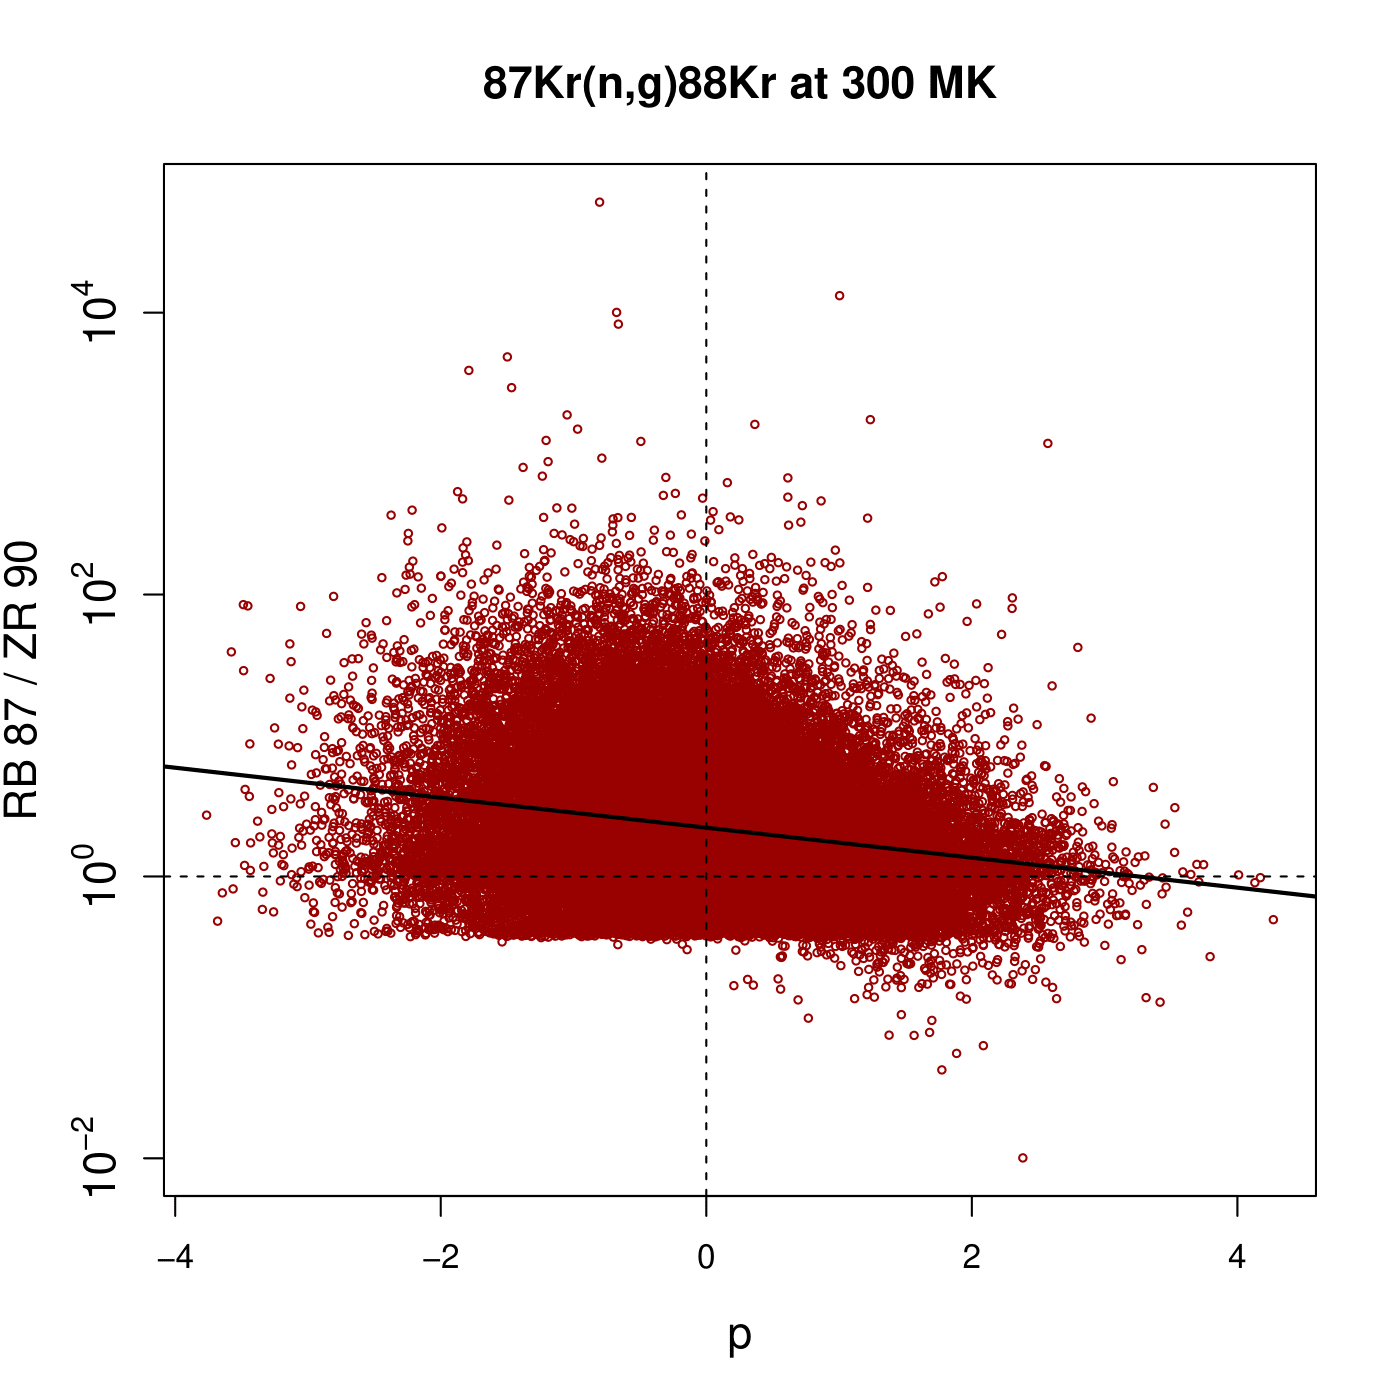
\includegraphics[width=\textwidth]{Chapter-3/figs/CorrRB87ZR90_87Kr_n_g_88Kr_300MK.png}
\end{subfigure}
\caption{\label{fig:Correlations_87Rb90Zr_ng}Correlations between the final mass fraction ratio $X(^{87}\mathrm{Rb})/X(^{90}\mathrm{Zr})$ and the four most important $(n,\gamma)$ reaction rates, ranked in the top 6 among all reactions by MI. See Fig. \ref{fig:Correlations_87Rb86Sr_ng} caption for details.}
\end{figure}

\subsubsection{The Neutron Sources}

Interestingly, the main neutron sources $^{13}\mathrm{C}(\alpha,n)^{16}\mathrm{O}$ and $^{22}\mathrm{N}(\alpha,n)^{25}\mathrm{Mg}$ do not make an appearance in Table \ref{tab:mutual_info}. In fact, they are mostly uncorrelated with either mass fraction ratio, as shown in the top two panels of Figs. \ref{fig:Correlations_87Rb86Sr_n} and \ref{fig:Correlations_87Rb90Zr_n} for $X(^{87}\mathrm{Rb})/X(^{86}\mathrm{Sr})$ and $X(^{87}\mathrm{Rb})/X(^{90}\mathrm{Zr})$, respectively. A possible explanation of this could be that these rates are already well-constrained, and sampling over a small uncertainty may not affect the nucleosynthesis. The $^{13}\mathrm{C}(\alpha,n)^{16}\mathrm{O}$ and $^{22}\mathrm{Ne}(\alpha,n)^{25}\mathrm{Mg}$ \texttt{Starlib} reaction rates at 300 MK have factor uncertainties of $f.u. = 1.183$ and $f.u. = 1.229$, respectively. In other words, using Eqn. \ref{eqn:lognorm_param}, $(f.u.)^{2} = x_{\mathrm{high}}/x_{\mathrm{low}} =$ 1.400 and 1.510, respectively. These are the ratios between the 84th and 16th percentiles of each reaction rate uncertainty. Compared to many rate uncertainties, this is quite small and could offer an explanation, even if these reactions do contribute to $^{87}$Rb abundance. Although the main neutron sources are not correlated, the $^{18}\mathrm{O}(\alpha,n)^{21}\mathrm{Ne}$ rate is mildly correlated with both ratios, according to Table \ref{tab:mutual_info}. This may act as an alternative neutron source.

\subsubsection{The Neutron Poisons}

We will now revisit the discussion of the $^{13}\mathrm{N}(n,p)^{13}\mathrm{C}$ and $^{14}\mathrm{N}(n,p)^{14}\mathrm{C}$ reactions. The known neutron poison $^{14}\mathrm{N}(n,p)^{14}\mathrm{C}$ makes an appearance in the top three correlations of Table \ref{tab:mutual_info}. However, it is counterintuitively associated with a positive correlation for both ratios from the $r_{s}$ signature. One should expect that the $^{86}$Rb and $^{85}$Kr s-process branchings are deactivated with decreasing neutron density. This troublesome situation is resolved when analyzing its scatter plot in the bottom left panel of Fig. \ref{fig:Correlations_87Rb86Sr_n} for nonlinear, non-monotonic correlations. This is a prime example of $r_{s}$ being potentially misleading. The correlation does not seem to be positive, and it may even be negative for negative $p$-values.

\begin{figure}[!p]
\centering
\begin{subfigure}[b]{0.495\textwidth}
\centering
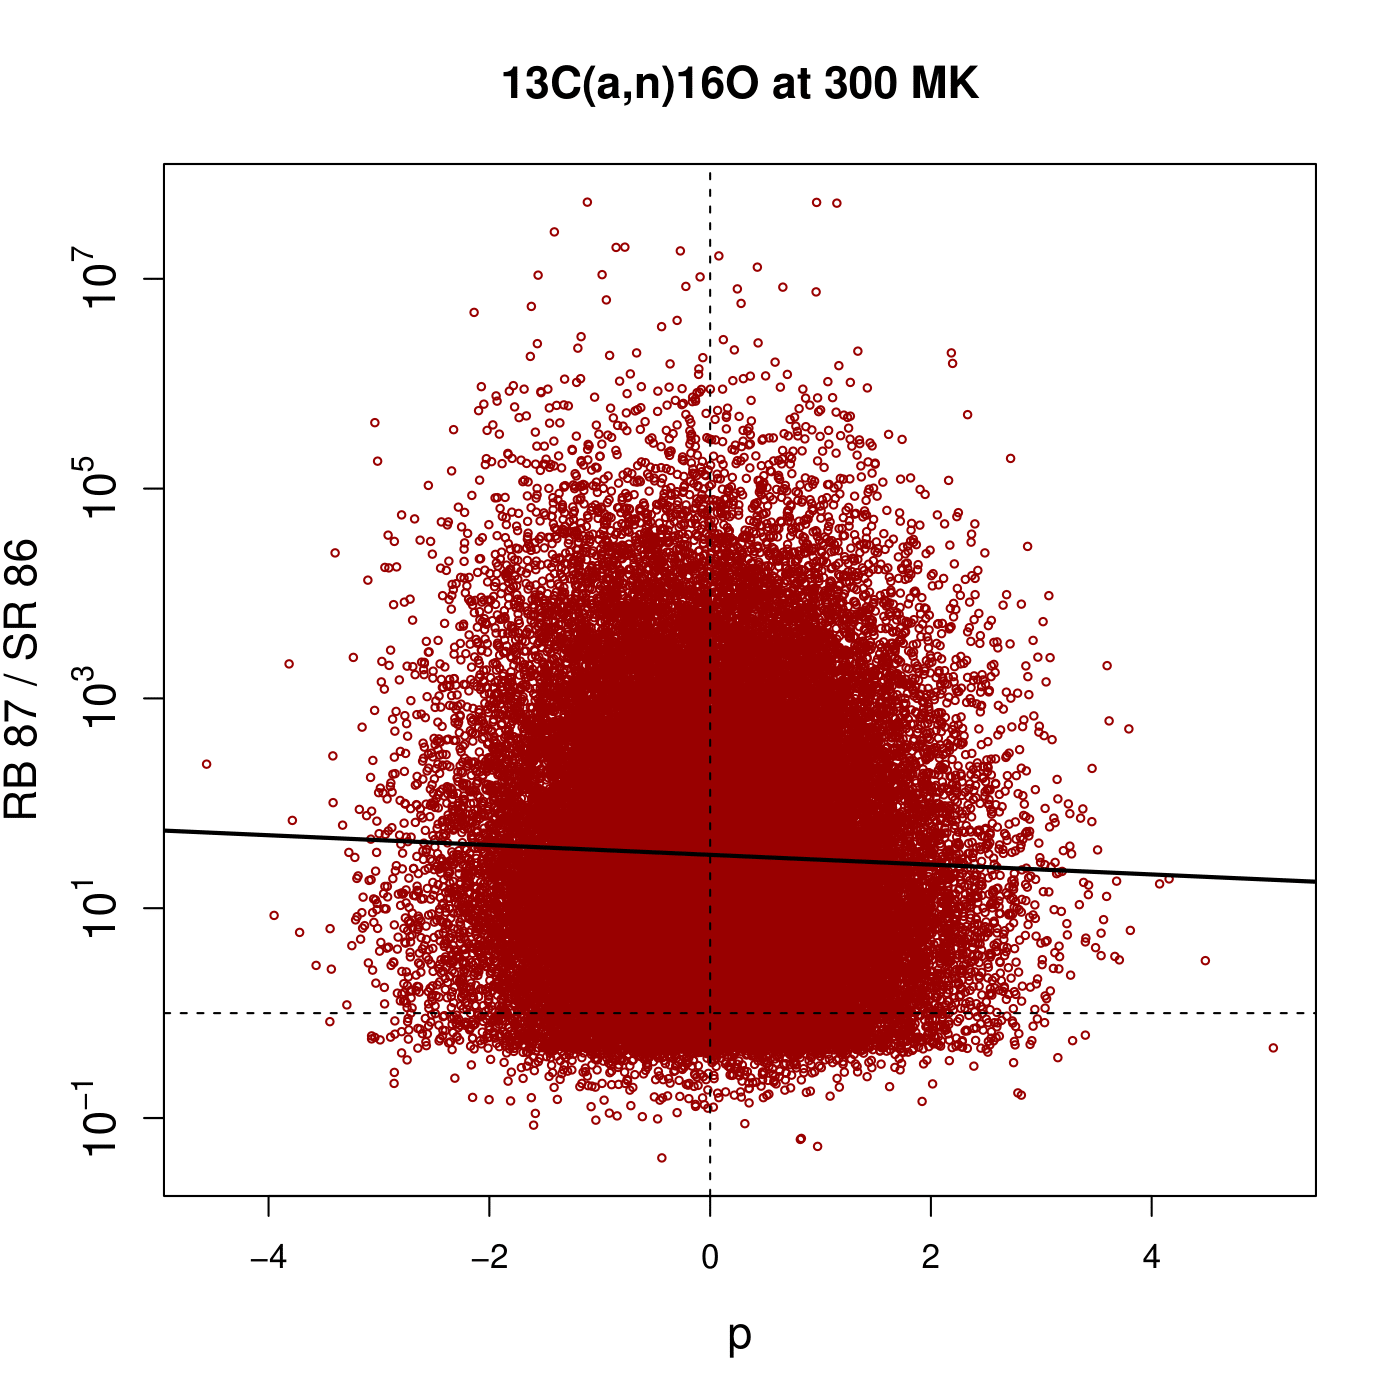
\includegraphics[width=\textwidth]{Chapter-3/figs/CorrRB87SR86_13C_a_n_16O_300MK.png}  
\end{subfigure}
\hfill
\begin{subfigure}[b]{0.495\textwidth}  
\centering 
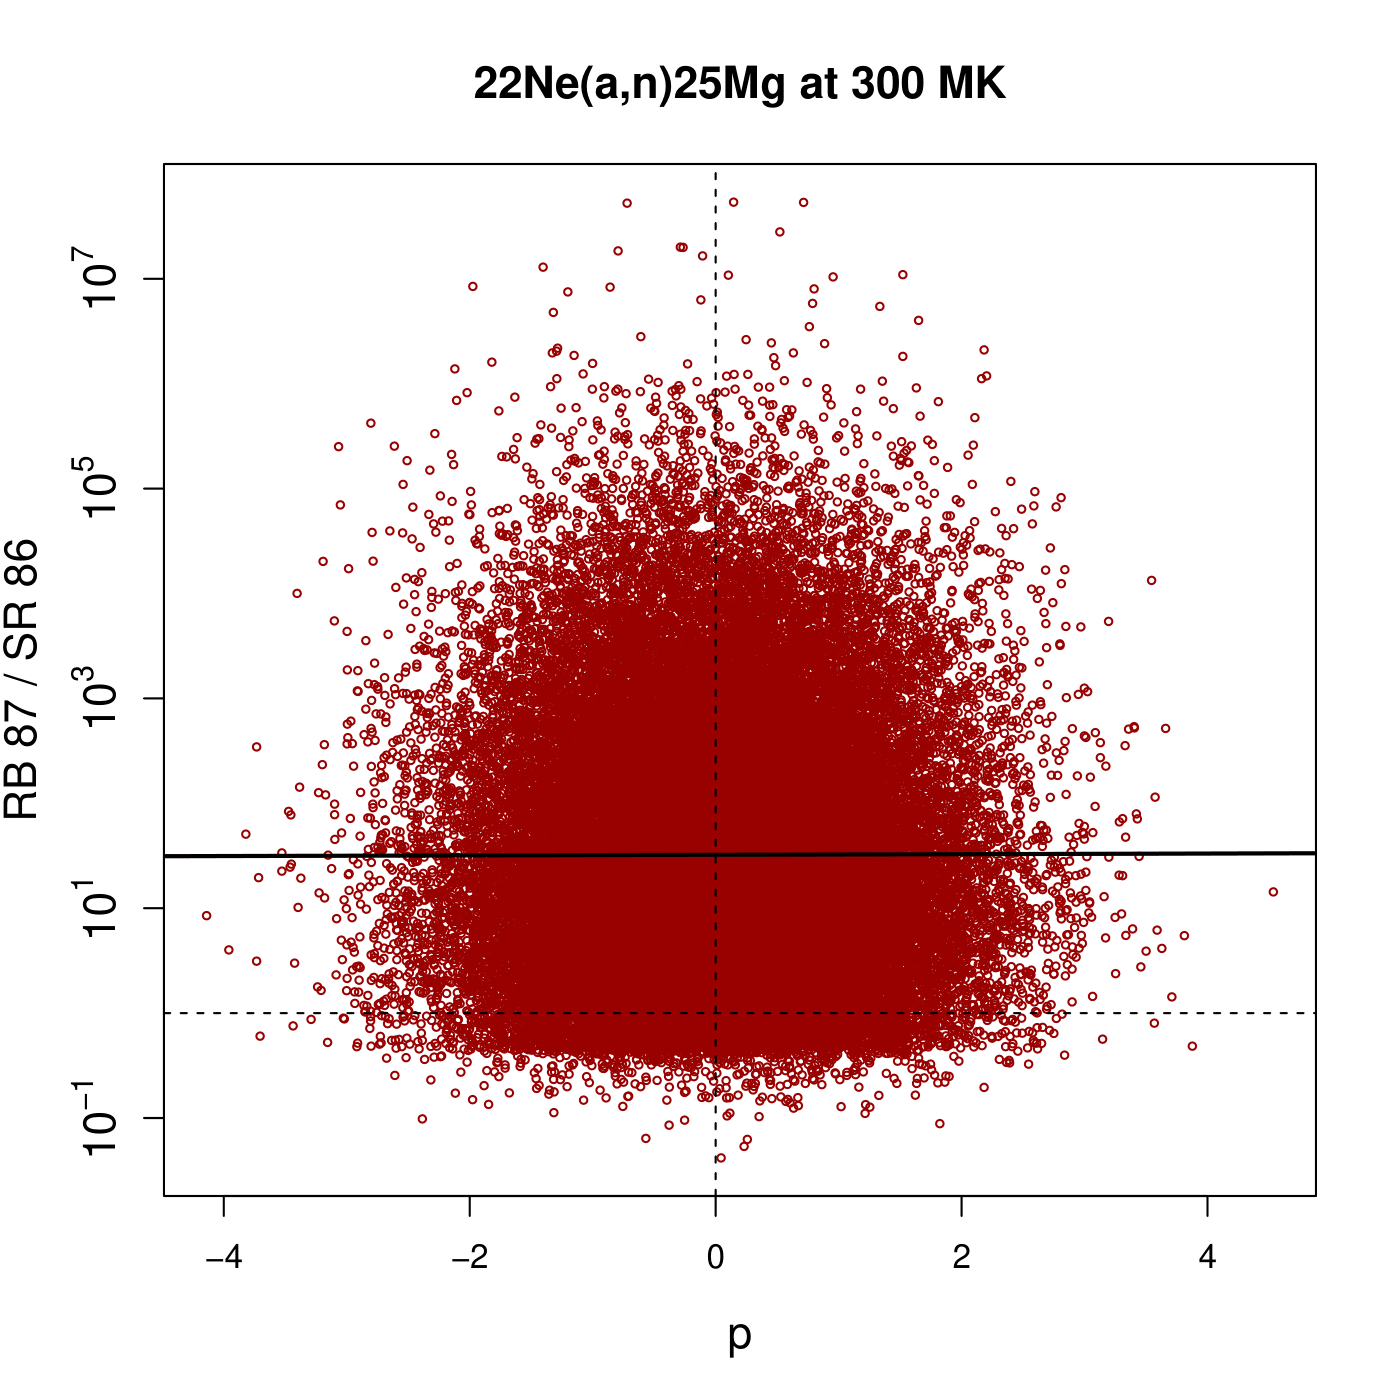
\includegraphics[width=\textwidth]{Chapter-3/figs/CorrRB87SR86_22Ne_a_n_25Mg_300MK.png}
\end{subfigure}
%\vskip\baselineskip
\begin{subfigure}[b]{0.495\textwidth}   
\centering 
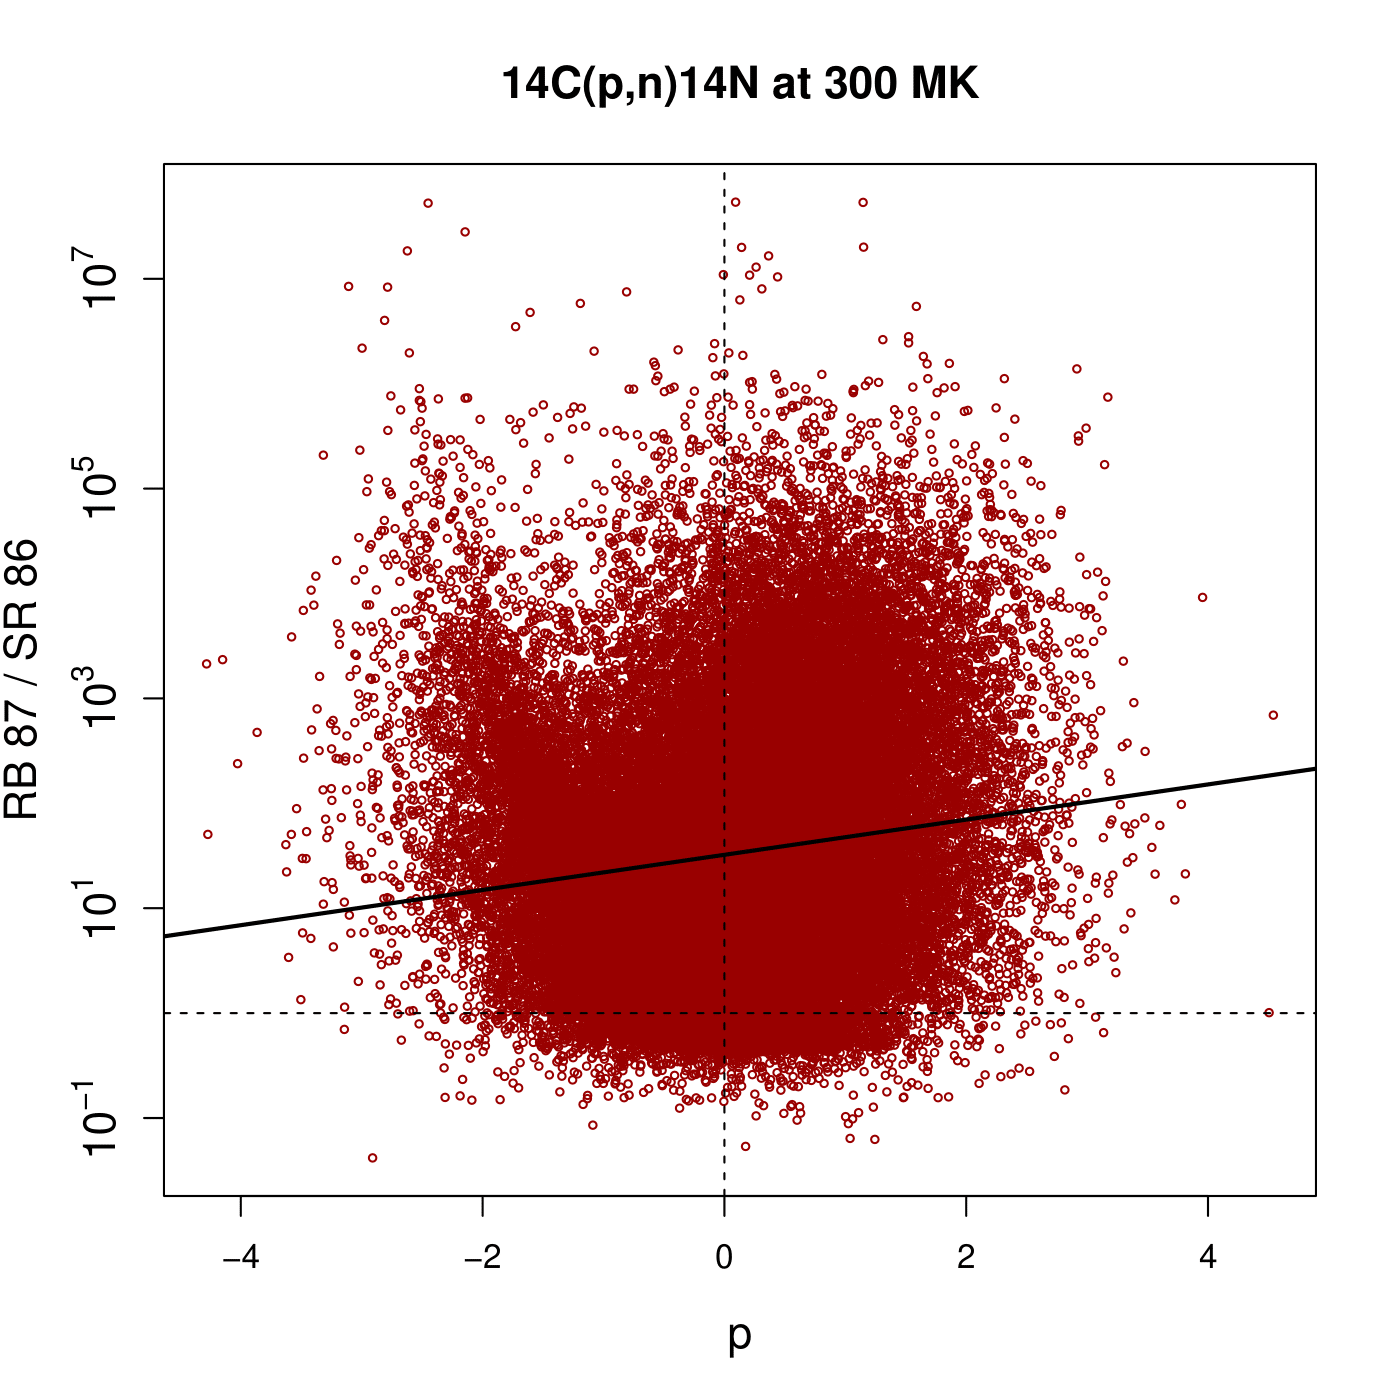
\includegraphics[width=\textwidth]{Chapter-3/figs/CorrRB87SR86_14C_p_n_14N_300MK.png}
\end{subfigure}
\hfill
\begin{subfigure}[b]{0.495\textwidth}   
\centering 
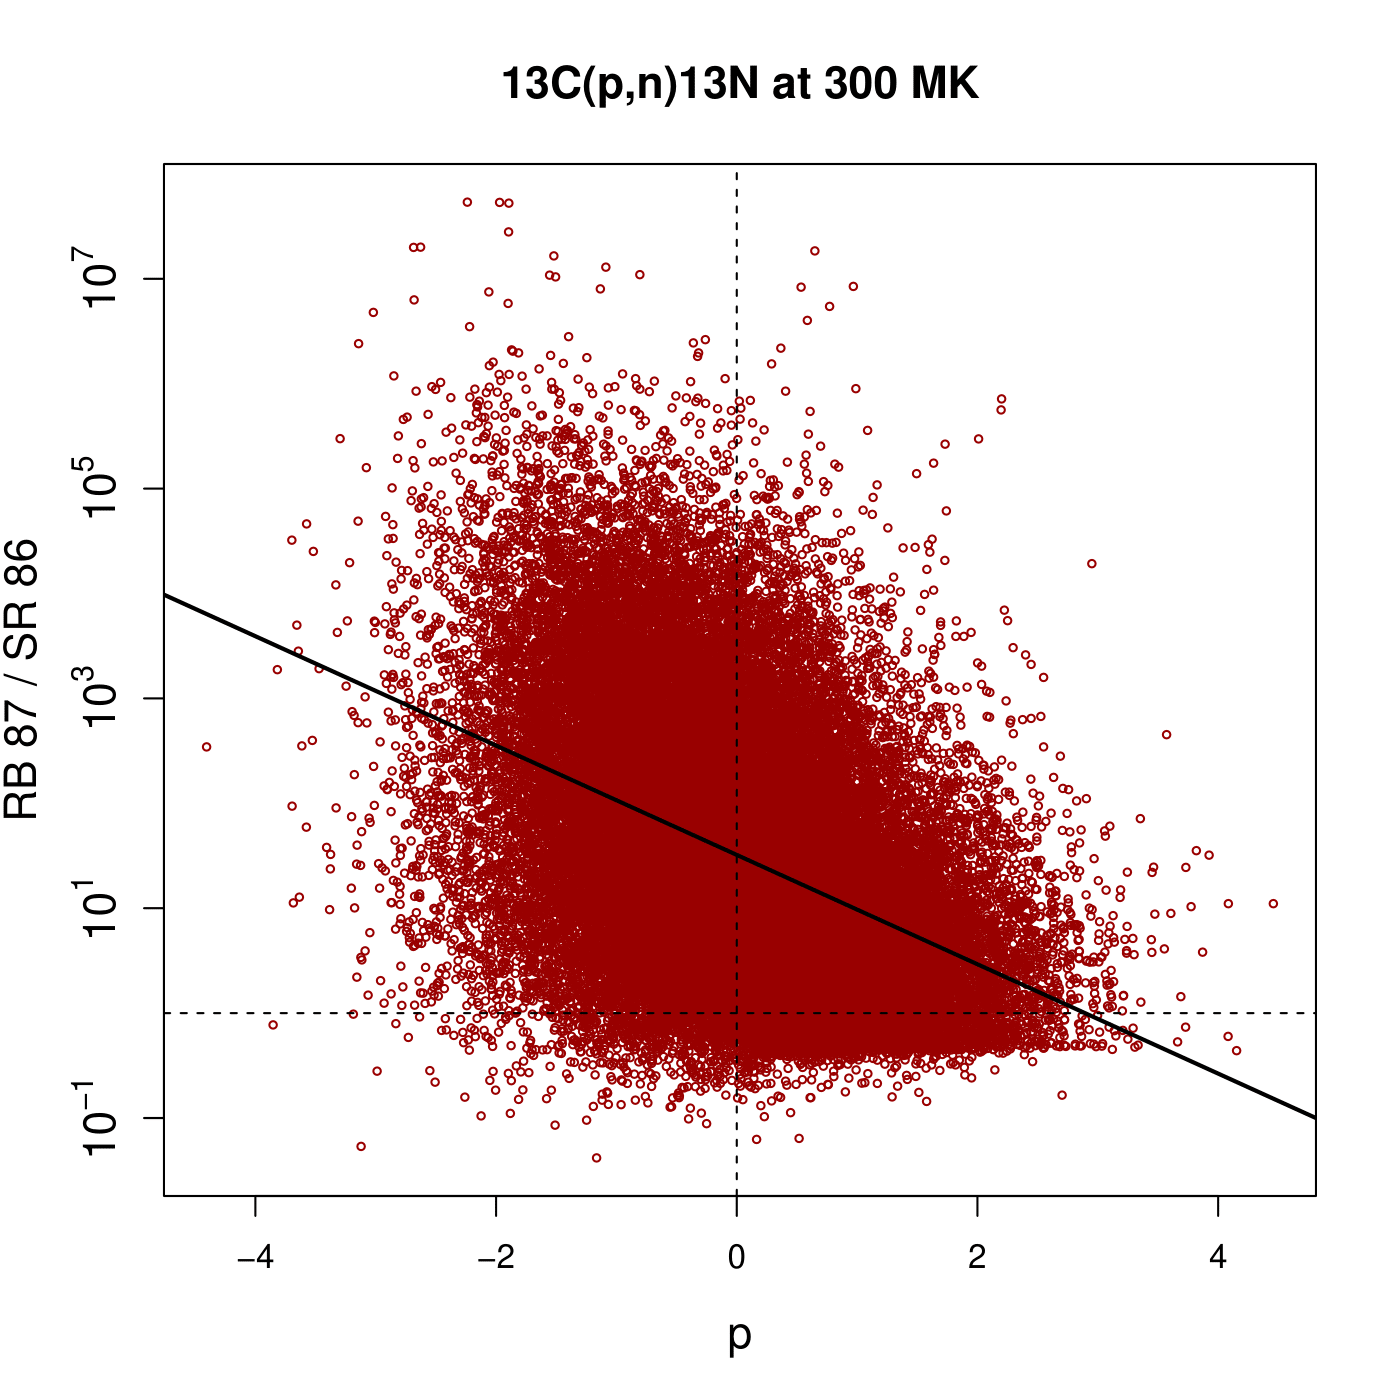
\includegraphics[width=\textwidth]{Chapter-3/figs/CorrRB87SR86_13C_p_n_13N_300MK.png}
\end{subfigure}
\caption{\label{fig:Correlations_87Rb86Sr_n}Correlations between the final mass fraction ratio $X(^{87}\mathrm{Rb})/X(^{86}\mathrm{Sr})$ and the reaction rates of the s-process neutron sources and neutron poisons. The neutron poisons $^{14}\mathrm{N}(n,p)^{14}\mathrm{C}$ and $^{13}\mathrm{N}(n,p)^{13}\mathrm{C}$ are labeled as their reverse reactions, which have equivalent correlations. See Fig. \ref{fig:Correlations_87Rb86Sr_ng} caption for details.}
\end{figure}

\begin{figure}[!p]
\centering
\begin{subfigure}[b]{0.495\textwidth}
\centering
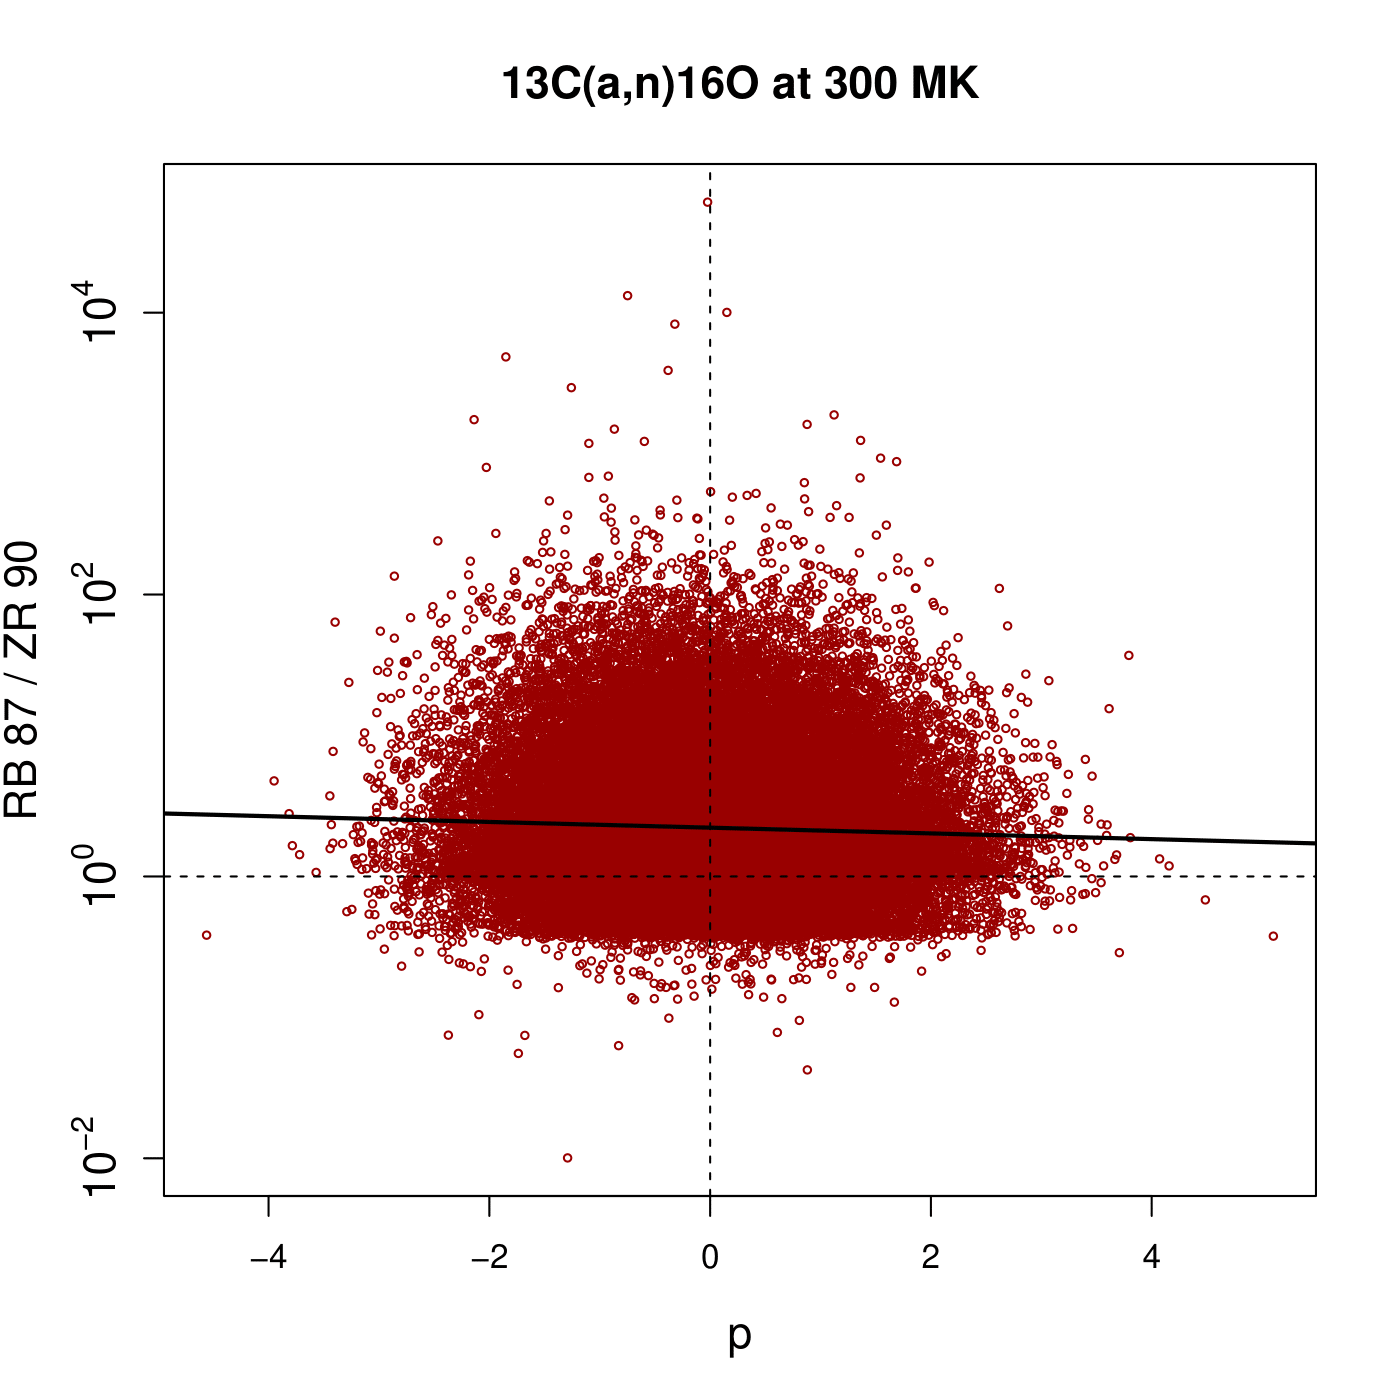
\includegraphics[width=\textwidth]{Chapter-3/figs/CorrRB87ZR90_13C_a_n_16O_300MK.png}  
\end{subfigure}
\hfill
\begin{subfigure}[b]{0.495\textwidth}  
\centering 
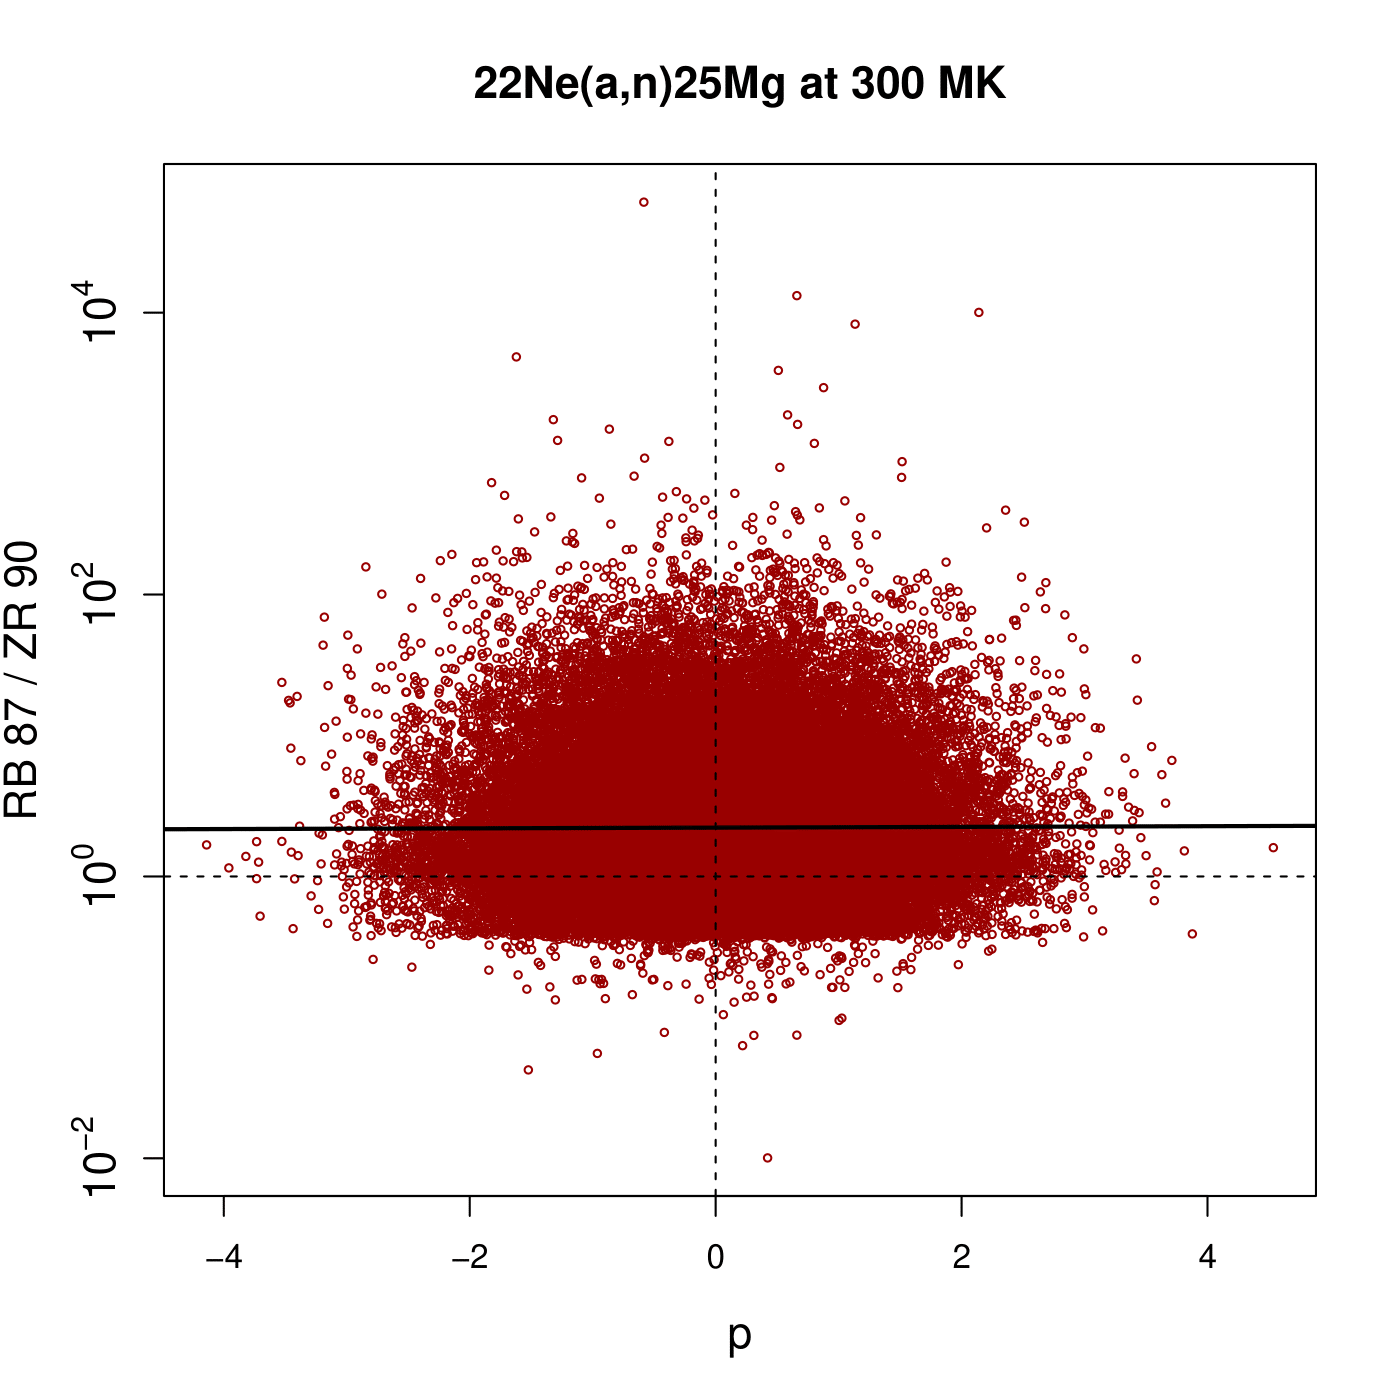
\includegraphics[width=\textwidth]{Chapter-3/figs/CorrRB87ZR90_22Ne_a_n_25Mg_300MK.png}
\end{subfigure}
%\vskip\baselineskip
\begin{subfigure}[b]{0.495\textwidth}   
\centering 
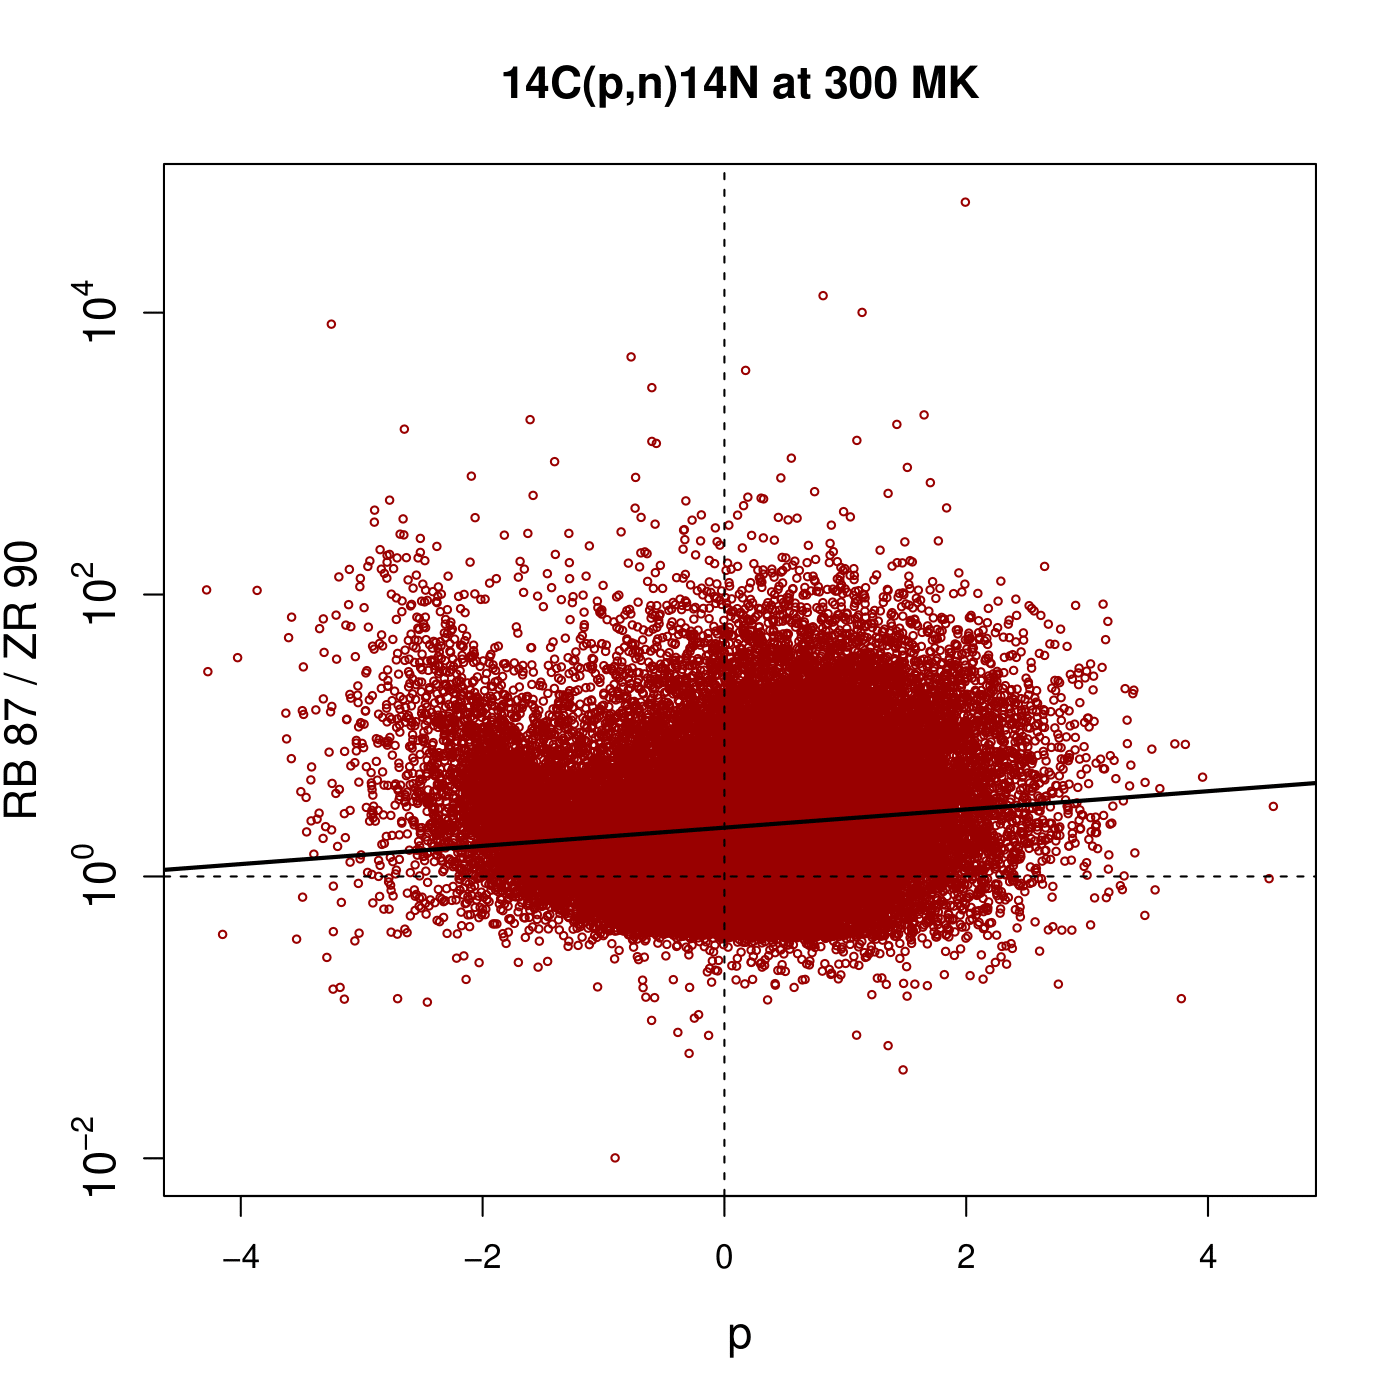
\includegraphics[width=\textwidth]{Chapter-3/figs/CorrRB87ZR90_14C_p_n_14N_300MK.png}
\end{subfigure}
\hfill
\begin{subfigure}[b]{0.495\textwidth}   
\centering 
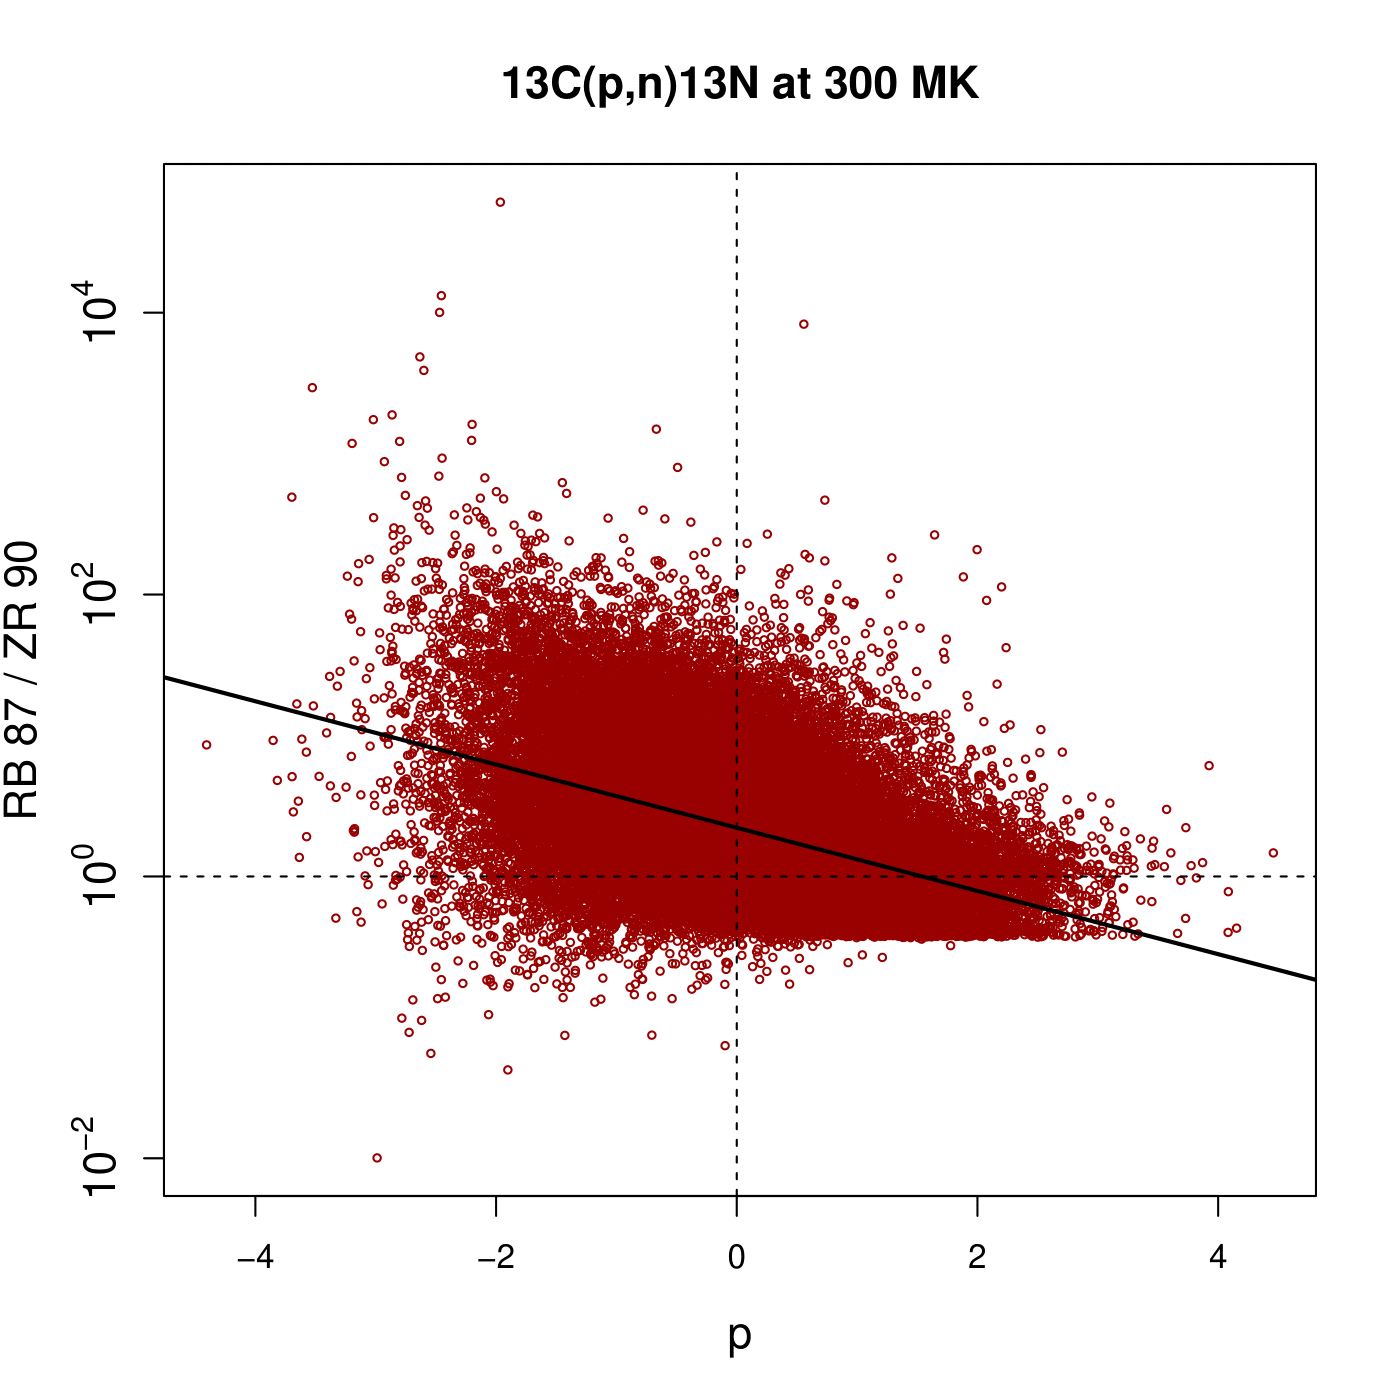
\includegraphics[width=\textwidth]{Chapter-3/figs/CorrRB87ZR90_13C_p_n_13N_300MK.png}
\end{subfigure}
\caption{\label{fig:Correlations_87Rb90Zr_n}Same as Fig. \ref{fig:Correlations_87Rb86Sr_n}, except with the final mass fraction ratio $X(^{87}\mathrm{Rb})/X(^{90}\mathrm{Zr})$. See Fig. \ref{fig:Correlations_87Rb86Sr_ng} caption for details.}
\end{figure}

Finally, the strength of the $^{13}\mathrm{N}(n,p)^{13}\mathrm{C}$ neutron poison correlation is somewhat surprising, as $^{14}\mathrm{N}(n,p)^{14}\mathrm{C}$ is the more well-documented neutron poison in the literature \cite{Habing2004}. It does have a strong negative $r_{s}$ correlation for both mass fraction ratios, which is not misleading in this case, as is clear in the scatter plots of Figs. \ref{fig:Correlations_87Rb86Sr_n} and \ref{fig:Correlations_87Rb90Zr_n} for $X(^{87}\mathrm{Rb})/X(^{86}\mathrm{Sr})$ and $X(^{87}\mathrm{Rb})/X(^{90}\mathrm{Zr})$, respectively. This reaction competes with the $^{13}\mathrm{N}(\beta^{+}\nu)^{13}\mathrm{C}$ reaction, leading to the same production of the $^{13}$C neutron source, but consuming neutrons in the process. In fact, Eqn. \ref{eqn:decay_constant} can be used to determine the conditions for which the $^{13}\mathrm{N}(n,p)^{13}\mathrm{C}$ rate is favored over $\beta^{+}$-decay. For $(n,p)$ to be favored, the neutron mass fraction $X_{n}$ would have to exceed
\begin{equation} \label{eqn:n_mass_frac_condition}
X_{n} > \frac{M_{n}}{\tau_{\beta^{+}}(^{13}\mathrm{N}) \rho N_{A} \langle \sigma v \rangle(T)} \approx 2.5 \times 10^{-15},
\end{equation}
where the mass density is $\rho = 10^{3}$ $\mathrm{g}/\mathrm{cm}^{-3}$; $M_{n}$ is the neutron mass; $\tau_{\beta^{+}}(^{13}\mathrm{N}) \approx 863$ s \cite{Audi2003} is the mean lifetime for $\beta^{+}$-decay, and the recommended $^{13}\mathrm{N}(n,p)^{13}\mathrm{C}$ reaction rate from \texttt{Starlib} at 300 MK is $N_{A} \langle \sigma v \rangle = 4.586 \times 10^{8}$ $\mathrm{cm}^{3}$ $\mathrm{s}^{-1}$ $\mathrm{mol}^{-1}$. Referring back to the abundance evolution for the single nucleosynthesis calculation shown in Fig. \ref{fig:abund_evol}, $X_{n}$ exceeds this amount initially with a value of $\approx 5 \times 10^{-14}$. At this $X_{n}$, the mean lifetime $\tau_{n}$ for $(n,p)$ is about $\tau_{n} \approx$ 43 s $<< 863$ s, confirming that $(n,p)$ is greatly favored. At its peak, $X_{n}$ is $8 \times 10^{-13}$, corresponding with $\tau_{n} \approx 3$ s, an even shorter mean lifetime. Eventually, $X_{n}$ drops to about $5 \times 10^{-18}$ in Figure \ref{fig:abund_evol}, which implies $\tau_{n} \approx 4.3 \times 10^{5}$ s $>> 863$ s. Therefore, the $\beta^{+}$-decay is finally favored at this point. This exercise shows that $^{13}\mathrm{N}(n,p)^{13}\mathrm{C}$ is surprisingly important for s-process nucleosynthesis and should be investigated further.

%\begin{figure}[t]
%\centering
%\begin{subfigure}[b]{0.495\textwidth}
%\centering
%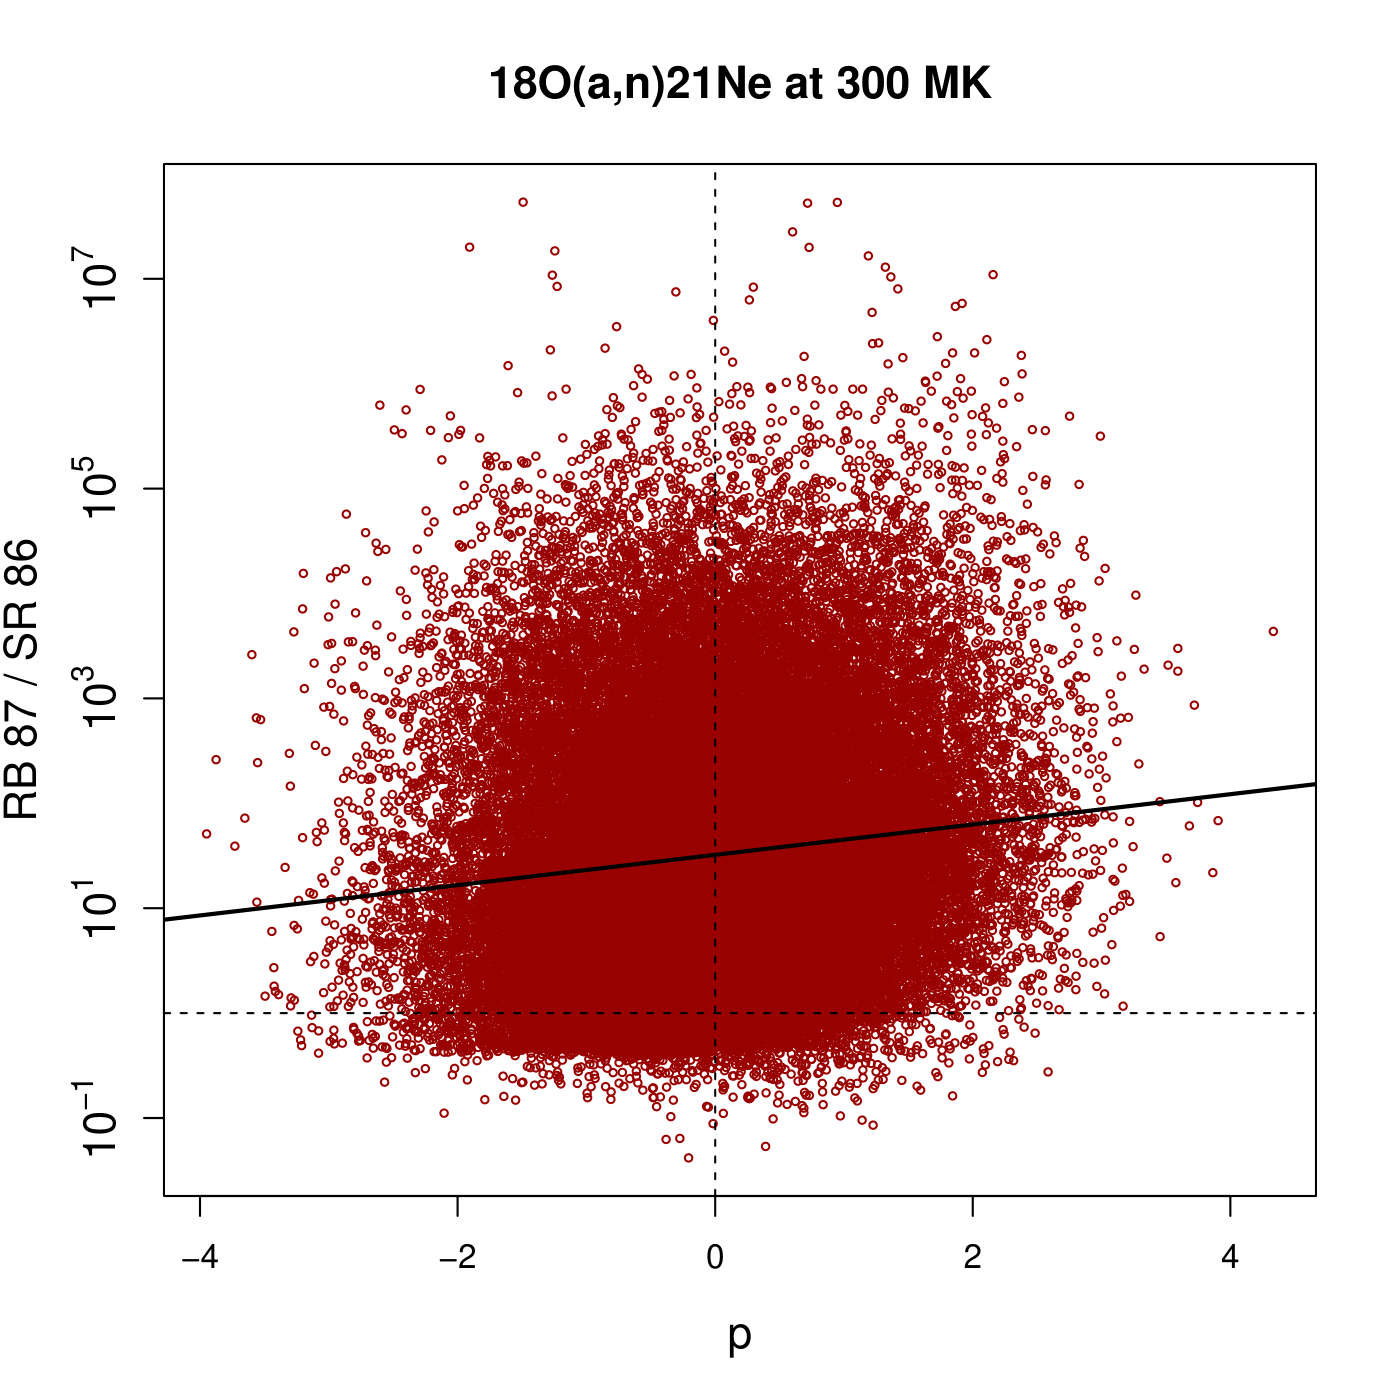
\includegraphics[width=\textwidth]{Chapter-3/figs/CorrRB87SR86_18O_a_n_21Ne_300MK.png}  
%\end{subfigure}
%\hfill
%\begin{subfigure}[b]{0.495\textwidth}  
%\centering 
%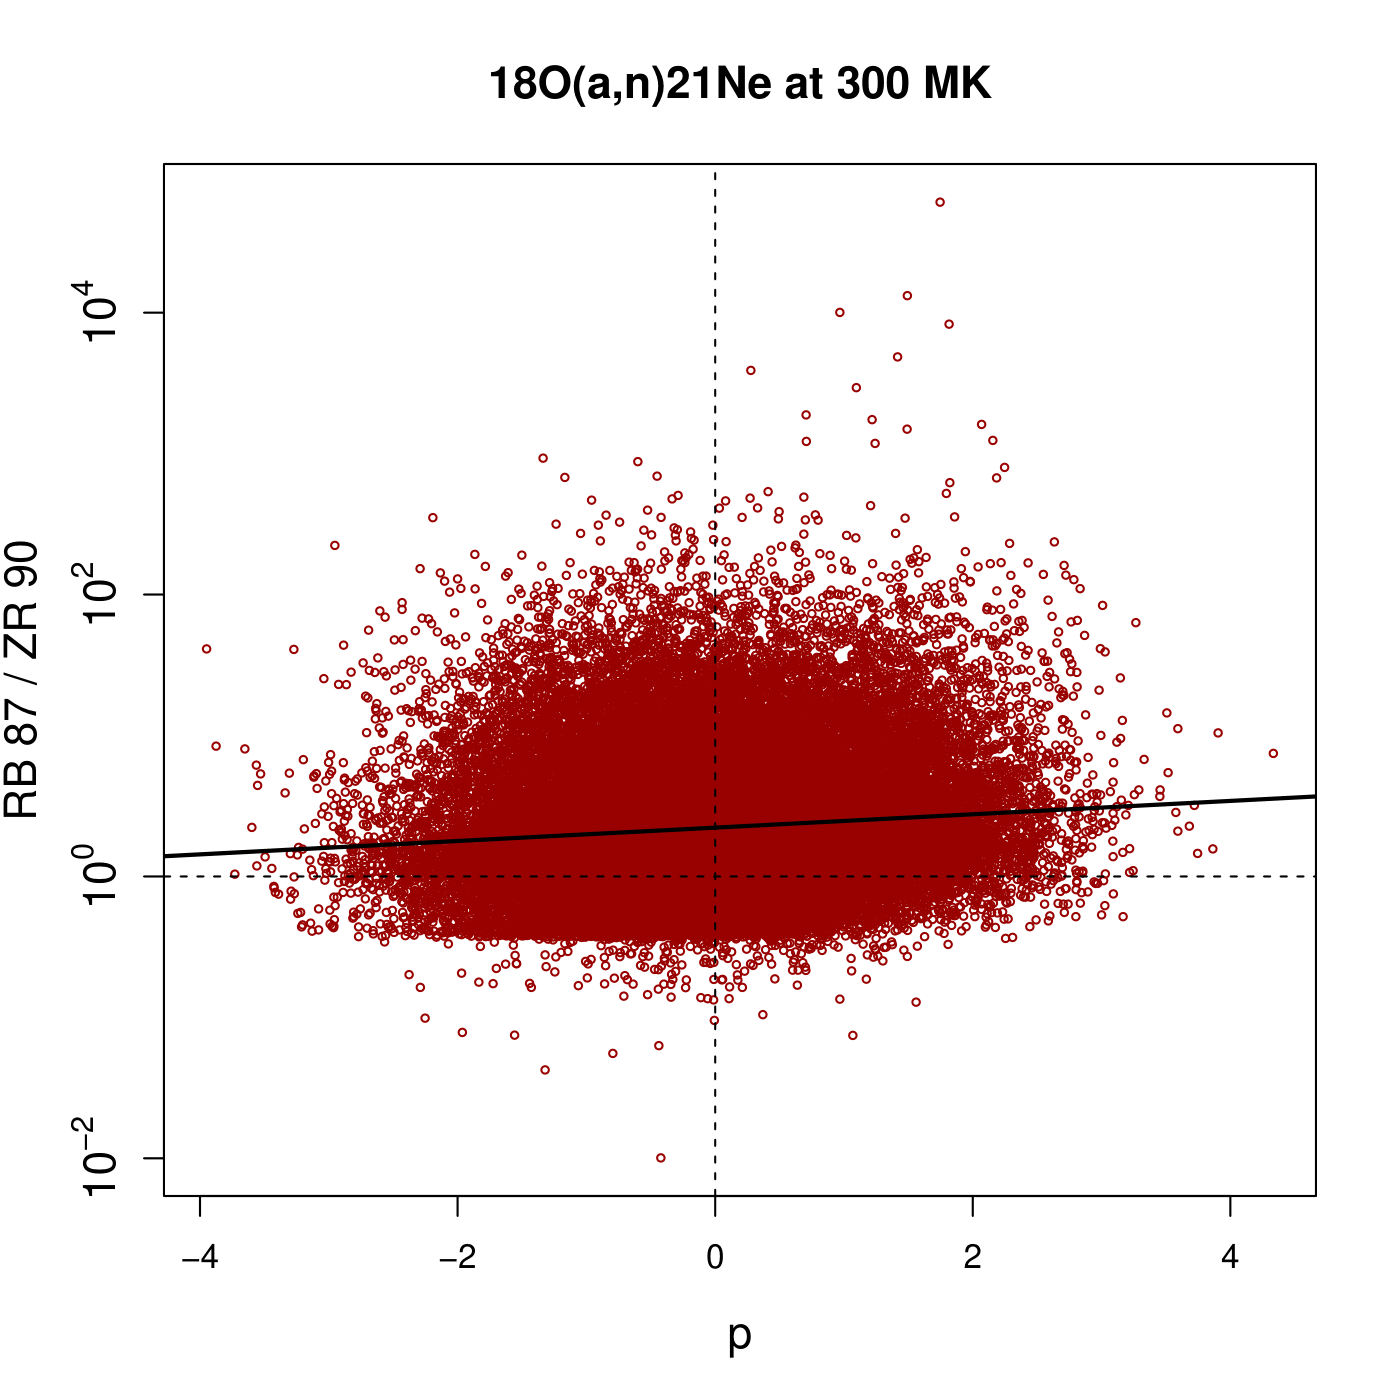
\includegraphics[width=\textwidth]{Chapter-3/figs/CorrRB87ZR90_18O_a_n_21Ne_300MK.png}
%\end{subfigure}
%\caption{\label{fig:Correlations_18O_a_n}Correlations between the final mass fraction ratio $X(^{87}\mathrm{Rb})/X_{i}$ and the reaction rate of the $^{18}\mathrm{O}(\alpha,n)^{21}\mathrm{Ne}$ neutron source, where $i$ represents $^{86}$Sr and $^{90}$Zr for the left and right plots, respectively. See Fig. \ref{fig:Correlations_87Rb86Sr_ng} caption for details.}
%\end{figure}

\subsection{The [Rb/Zr], [Rb/Sr], and [Rb/Fe] Ratios}

Not only can the isotopic ratios $X(^{87}\mathrm{Rb})/X(^{86}\mathrm{Sr})$ and $X(^{87}\mathrm{Rb})/X(^{90}\mathrm{Zr})$ be investigated; the elemental ratios $X(\mathrm{Rb})/X(\mathrm{Sr})$ and $X(\mathrm{Rb})/X(\mathrm{Zr})$ can be probed as well. Analysis of these ratios leads to similar conclusions drawn in Section \ref{subsec:Corr}, and the correlation plots for the elemental ratios are omitted for this reason. The main differences are for specific reactions such as $^{90}\mathrm{Y}(n,\gamma)^{91}\mathrm{Y}$ and $^{90}\mathrm{Y}(\beta^{-}\nu)^{90}\mathrm{Zr}$, which are no longer as sensitive. Both of these reactions inevitably lead to Zr. Even though the $(n,\gamma)$ reaction bypasses $^{90}$Zr, it produces $^{91}$Zr, and Zr has several stable isotopes up to $^{96}$Zr. Overall, however, most reaction rates sensitive to the isotopic ratios are also sensitive to the elemental ratios. This is especially true for the $(n,\gamma)$ reactions and $\beta^{-}$-decays of the $^{86}$Rb and $^{85}$Kr s-process branchings, as well as the $^{13}\mathrm{N}(n,p)^{13}\mathrm{C}$ and $^{14}\mathrm{N}(n,p)^{14}\mathrm{C}$ neutron poisons.

An illuminating result comes from the probability densities of the final elemental abundances in the form of Eqn. \ref{eqn:abundance}, calculated relative to solar system abundances. This equation is used for each reaction network sample to determine the range of possible [Rb/Sr] and [Rb/Zr] ratios, as well as Rb abundances ([Rb/Fe]) resulting from simultaneously sampling every reaction rate uncertainty. Figure \ref{fig:RbZr_Hist} showcases these results, where the $x$-axis is in terms of dex. By definition, 0 dex implies that the ratio consists of relative solar system abundances. The initial Rb, Sr, and Zr isotopic mass fractions were all given relative solar system abundances. The initial [Rb/Sr] and [Rb/Zr] ratios were therefore roughly 0 dex, and the figure shows that there was little overall change in these relative abundances after the Monte Carlo network calculation.

However, the initial $^{56}$Fe mass fraction was enhanced from its solar system value (see Table \ref{tab:init_abunds}). The initial [Rb/Fe] abundance before the calculation was -0.918 dex. Assuming this variation from initial solar system abundances did not play a significant role in the nucleosynthesis, the [Rb/Fe] probability density can be corrected to account for its initial -0.918 dex value. This assumption was tested in an additional Monte Carlo network calculation for $10^{3}$ samples with an initial solar system $^{56}$Fe mass fraction. No significant differences were found in both the elemental and isotopic mass fraction ratio probability densities. Hence, the [Rb/Fe] probability density has been translated by +0.918 dex in Fig. \ref{fig:RbZr_Hist}. This corrected [Rb/Fe] result shows that the Rb abundance has increased slightly ($\sim +7\%$).
%, and the mean of the final [Rb/Fe] probability density is -0.89 dex, an increase of +0.03 dex ($\sim +7\%$).

\begin{figure}[t]
\centering
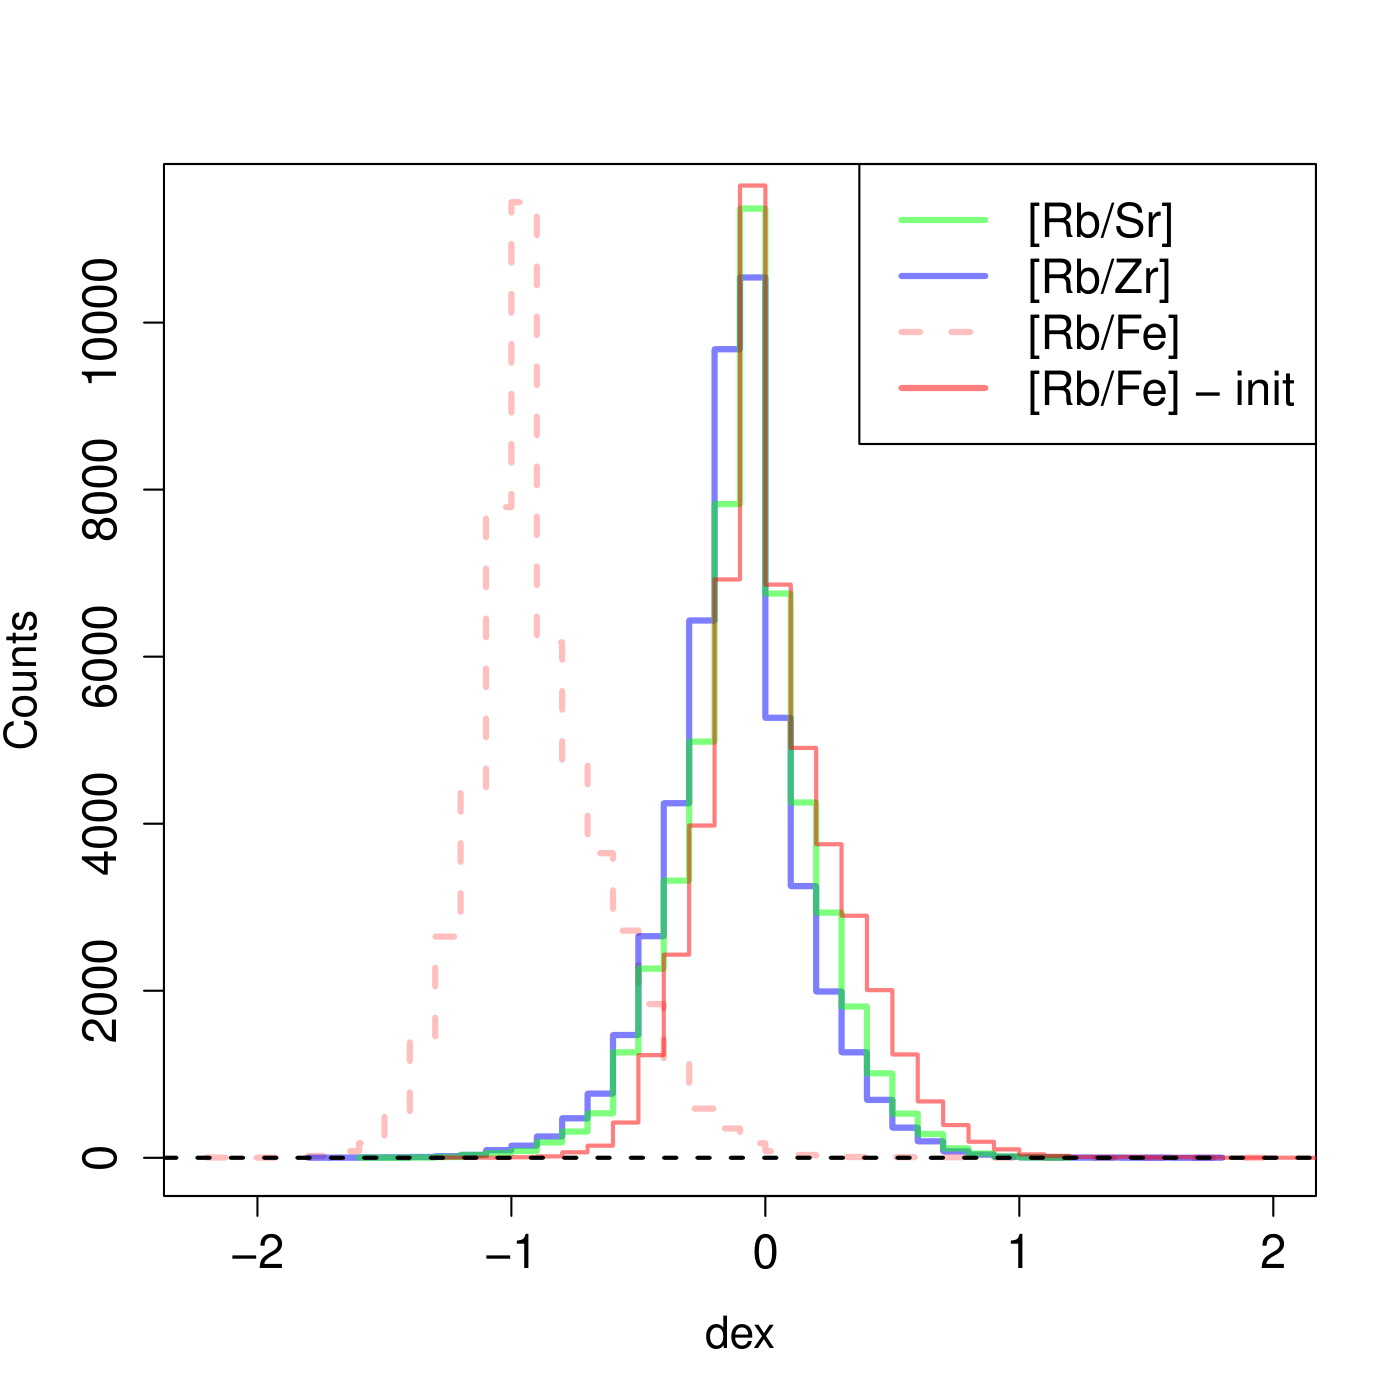
\includegraphics[width=4.55in]{Chapter-3/figs/Hist_Ele_Dex_Ratio_ModFe.png}
\caption{\label{fig:RbZr_Hist}Probability densities of the [Rb/Sr] (green), [Rb/Zr] (blue) and [Rb/Fe] (red, faded) abundance ratios resulting from the Monte Carlo reaction network calculation for $5 \times 10^{4}$ samples at $T = 300$ MK, $\rho = 10^{3}$ $\mathrm{g}/\mathrm{cm}^{3}$, and $X_{\mathrm{last}}(^{4}\mathrm{He}) = 0.7$, with $X_{\mathrm{init}}(^{4}\mathrm{He}) = 0.75$. The solid red probability density was obtained by correcting [Rb/Fe] for its enhanced $^{56}$Fe initial mass fraction relative to solar system abundance. $[\mathrm{Rb}/\mathrm{Fe}]_{\mathrm{init}}$ refers to the initial value of [Rb/Fe] before the network calculation (see text).}
\end{figure}

\begin{table}[t]
\centering
\caption{\label{tab:Prob_Dens}Percentiles from $-2\sigma$ to $+2\sigma$ of the [Rb/Sr], [Rb/Zr], and [Rb/Fe] probability densities from the present Monte Carlo reaction network calculation.}
\begin{tabular}{cccccc}
\hline\midrule
{}&2.5$\%$&16$\%$&50$\%$&84$\%$&97.5$\%$\\ \midrule
$[\mathrm{Rb}/\mathrm{Sr}]$&-0.594&-0.301&-0.061&0.167&0.468\\
$[\mathrm{Rb}/\mathrm{Zr}]$&-0.667&-0.348&-0.112&0.098&0.418\\
$[\mathrm{Rb}/\mathrm{Fe}]$&-0.442&-0.206&-0.016&0.288&0.622\\
\hline\hline
\end{tabular}
\end{table}

The median, $\pm 1\sigma$ percentiles, and $\pm 2\sigma$ percentiles of the [Rb/Sr], [Rb/Zr], and [Rb/Fe] probability densities are listed in Table \ref{tab:Prob_Dens}. Comparing to the s-process nucleosynthesis models of Refs. \cite{Karakas2012,Raai2012,Karakas2016,Pignatari2016} in Fig. \ref{fig:RbProblem}, the [Rb/Fe] and [Rb/Zr] probability densities of the present analysis span almost all of these models, within $\pm 2\sigma$. The only exceptions are the models that use an artificially delayed superwind (green and red) to enhance the Rb abundance. The probability densities also simultaneously agree with most of the range of observations, shown by the blue shading in Fig. \ref{fig:RbProblem}. However, like the other models, this reaction rate sensitivity study does not explain the largest observed [Rb/Zr] ratios. It also does not reproduce the largest observed [Rb/Fe] abundances.

\subsection{Discussion}

As mentioned in Refs. \cite{Raai2012,Perez2017}, a potential scenario that may offer an explanation for the remaining discrepancies is that Zr could be condensed into dust in the stellar atmosphere. Observations sample the gas around a star, not the dust. Therefore, if Zr is depleted by condensing into dust, and Rb is not, this could be the mechanism behind these high observed [Rb/Zr] ratios. In fact, Zr has a condensation temperature over twice as large as Rb \cite{Raai2012}, making it easier to condense. Models of dust formation could offer a solution.

One area that the present analysis did not cover is the sensitivity of systematic reaction rate variations. Sampling the reaction rates within their uncertainties assumes those uncertainties are properly described. If some of the key rates, e.g. the neutron sources $^{13}\mathrm{C}(\alpha,n)^{16}\mathrm{O}$ and $^{22}\mathrm{Ne}(\alpha,n)^{25}\mathrm{Mg}$ were systematically altered beyond their established uncertainties, the discrepancy might be explained. Unknown systematic uncertainties are often associated with experimentally constrained reaction rates, so this should be a topic of investigation.

%\section{The $^{86}\mathrm{\textbf{Rb}}(n,\gamma)^{87}\mathrm{\textbf{Rb}}$ Reaction Rate} \label{sec:86Rb_n_g_rate}

%\subsection{Recent Constraint with Nuclear Resonance Fluorescence}

% NRF measurement at HIGS (monoenergetic photons) and $\gamma$ELBE (Bremsstrahlung). Show the PSF and NLD. The NLD is still uncertain. The 86Sr(p,g)87Rb proton-capture reaction would help, and the 86Rb(3He,d)87Rb could be performed too.

%\subsection{The $^{86}\mathrm{\textbf{Kr}}(p,\gamma)^{87}\mathrm{\textbf{Rb}}$ and $^{86}\mathrm{\textbf{Kr}}(^{3}\mathrm{\textbf{He}},d)^{87}\mathrm{\textbf{Rb}}$ Reactions}

% The 87Rb NRF paper mentions 86Kr(p,g)87Rb as a way of reducing the level 

\section{Conclusions}

The ``rubidium problem'' was investigated with the results of a Monte Carlo reaction network calculation, where every reaction rate uncertainty in the network was sampled simultaneously. Final abundance probability densities were extracted for the key nuclei affected by the $^{86}$Rb and $^{85}$Kr s-process branchings. Ratios of $^{87}$Rb/$^{86}$Sr and $^{87}$Rb/$^{90}$Zr were found to be correlated with several key reaction rates. Namely, $^{86}\mathrm{Rb}(n,\gamma)^{87}\mathrm{Rb}$, $^{13}\mathrm{N}(n,p)^{13}\mathrm{C}$, and $^{14}\mathrm{N}(n,p)^{14}\mathrm{C}$ were the 3 reaction rates most correlated with these ratios, indicating that these rates are significant to s-process nucleosynthesis and Rb abundance in particular. The other $(n,\gamma)$ reactions and $\beta^{-}$-decays associated with the $^{86}$Rb and $^{85}$Kr s-process branchings were also found to be significant. However, the neutron sources $^{13}\mathrm{C}(\alpha,n)^{16}\mathrm{O}$ and $^{22}\mathrm{Ne}(\alpha,n)^{25}\mathrm{Mg}$ were found to not be correlated with Rb abundance. This does not mean that neither of these sources were activated, but it does suggest that their rate uncertainties are not significant in altering s-process nucleosynthesis at $T = 300$ MK, the transition temperature determining the dominant neutron source.

The [Rb/Zr] and [Rb/Fe] probability densities from the present Monte Carlo reaction network were mostly found to be in agreement with the models of Refs. \cite{Karakas2012,Raai2012,Karakas2016,Pignatari2016}, except for the cases where Rb abundance was artificially enhanced. Much of the [Rb/Zr] and [Rb/Fe] observations of Ref. \cite{Perez2017} were also reproduced, except for large ratios of $\gtrsim$ 0.4 dex and $\gtrsim$ 0.6 dex, respectively. The model-observation discrepancy is therefore still present for [Rb/Zr] ratios between 0.6-1.05 dex, and reaction rate uncertainties are likely not the solution.